% Methodology

\begin{figure}
    \centering
    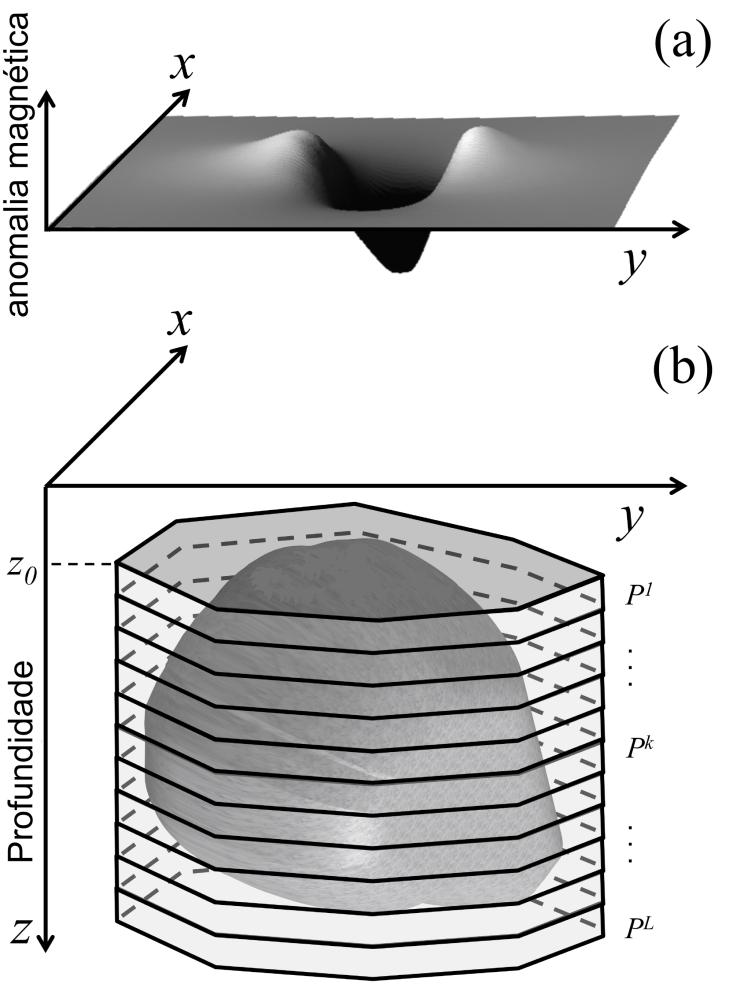
\includegraphics[scale=1]{figures/observed_data.png}
    \caption{Schematic representation (modified from \cite{oliveirajr-barbosa2013}) of (a) total-filed anomaly (gray surface) produced by (b) a 3-D anomalous source (dark gray volume). The interpretation model in (b) consists of a set of L vertical, juxtaposed 3-D prisms $P^k$ , $k = 1,\dots, L$, (light gray prisms) in the vertical direction of a right-handed coordinate system.}
    \label{fig:obs}
\end{figure}

\begin{figure}
    \centering
    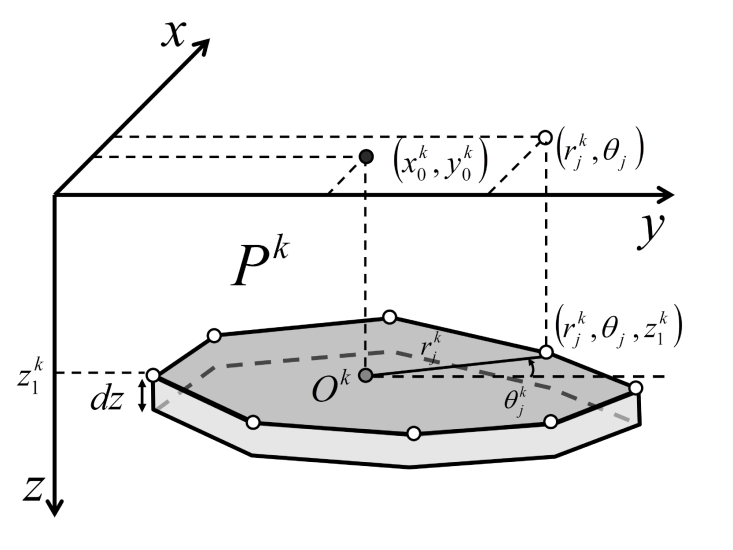
\includegraphics[scale=0.3]{figures/prism_parameters_mod.png}
    \caption{Polygonal cross-section of the $k$th vertical prism described by $V$ vertices (white dots) with radii $r^k_j$, $j = 1, \dots, V$, $k = 1, \dots, L$ , referred to an arbitrary origin $O^k$ (grey dot) with horizontal Cartesian coordinates ($x_0^k$ , $y_0^k$), $k = 1, \dots, L$ , (black dot).}
    \label{fig:prism_parameters}
\end{figure}

% Application to synthetic data - simple model

\begin{figure}
    \centering
    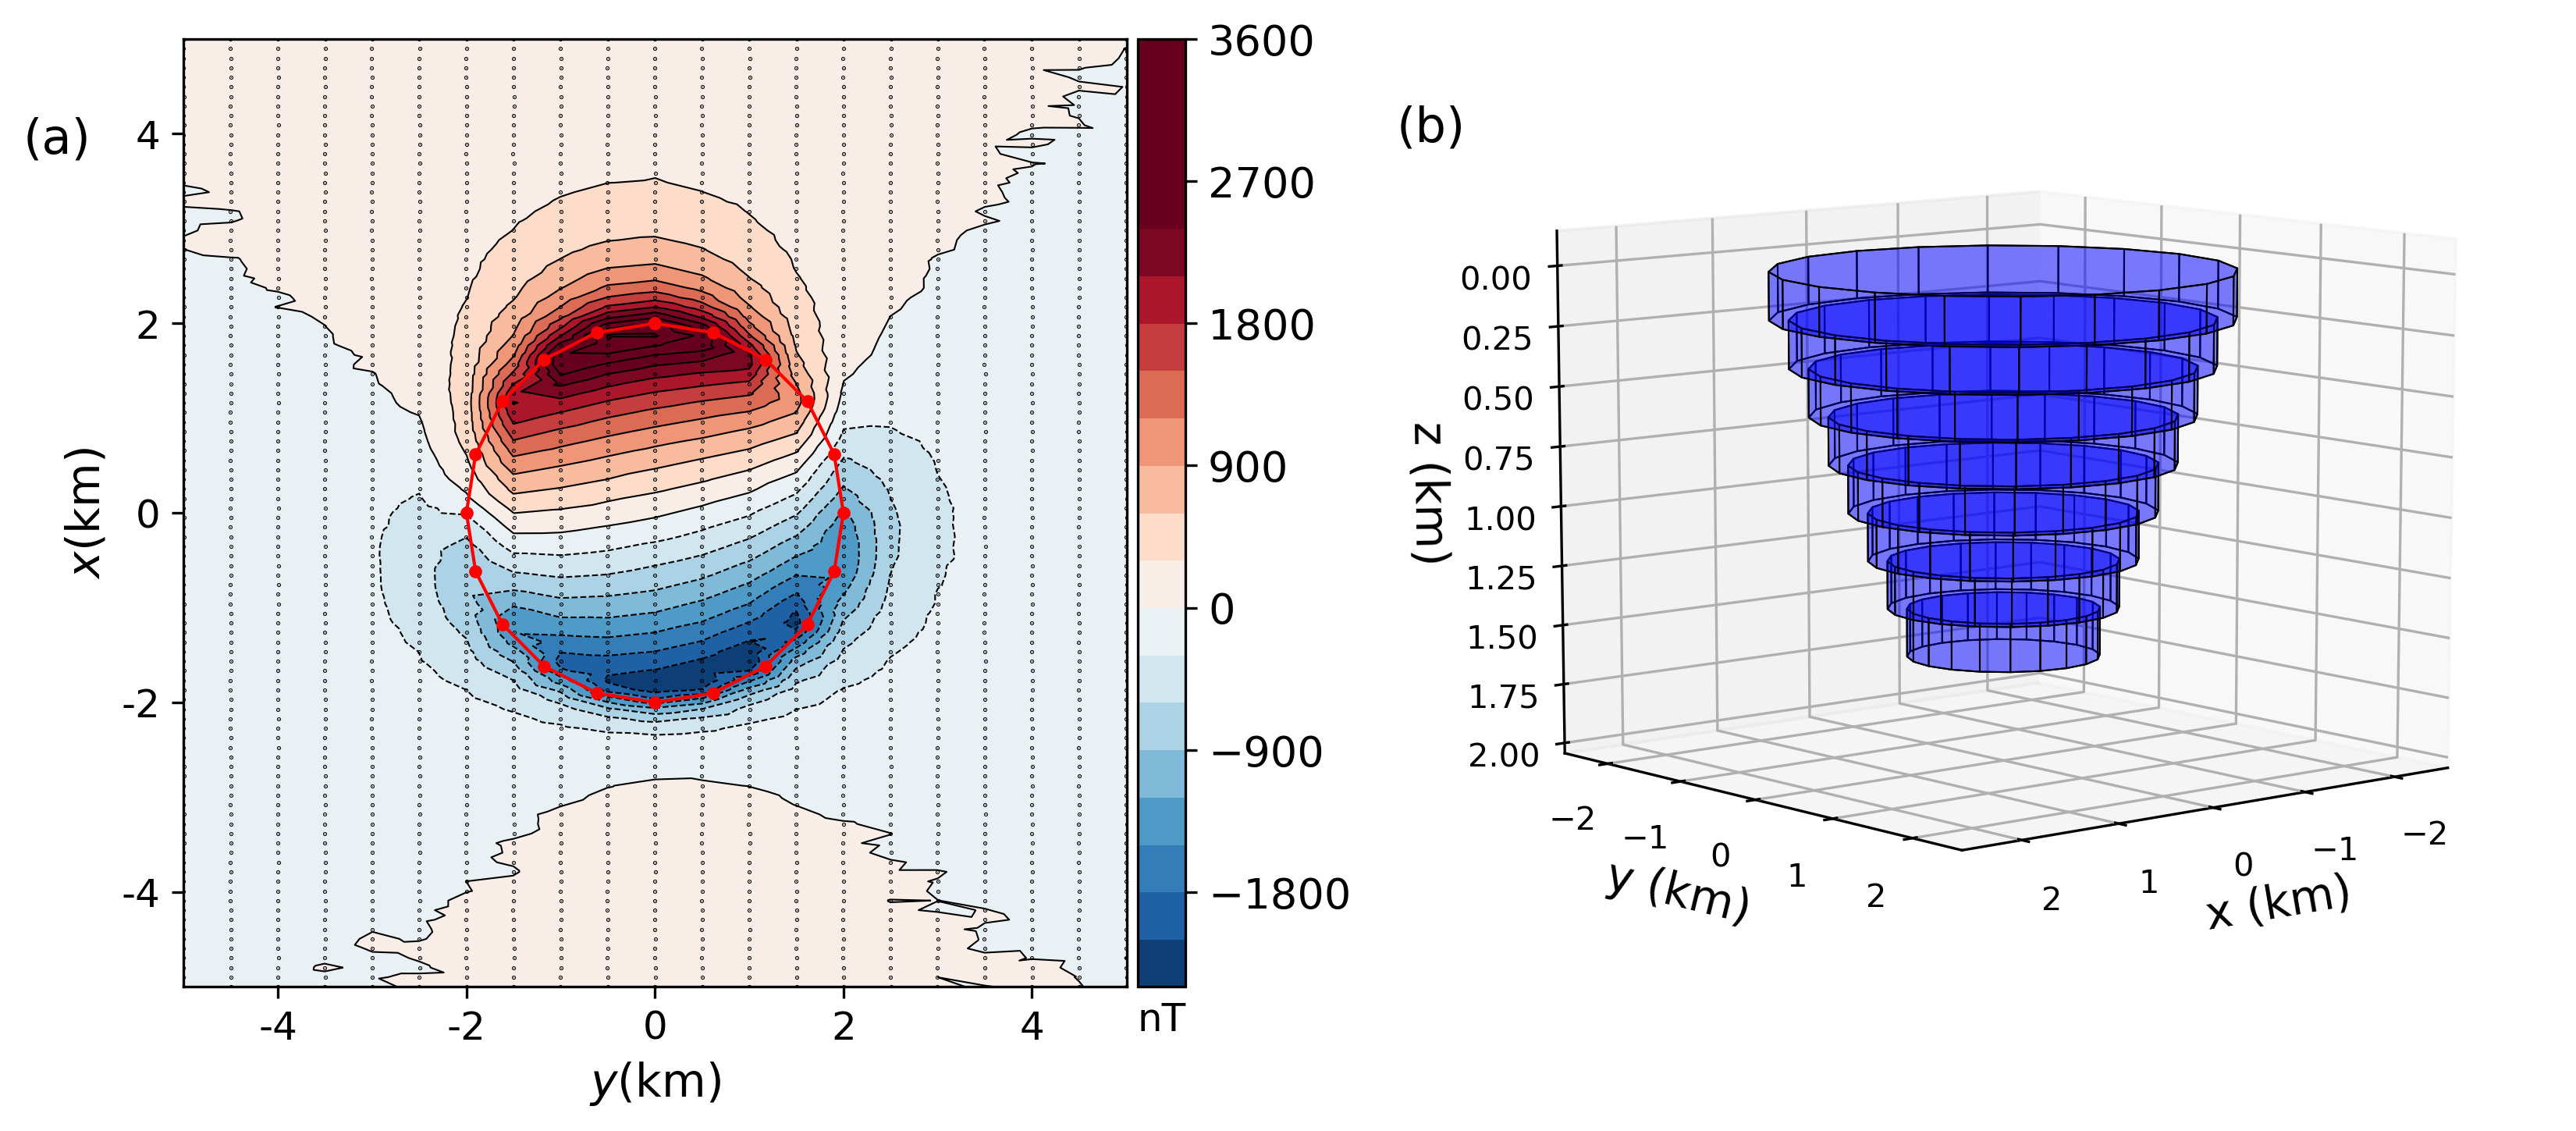
\includegraphics[width=\linewidth]{figures/simple_model_data.png}
    \caption{Simple model simulation. (a) Noise-corrupted total-field anomaly produced by the lopolithic-like body (blue prisms) shown in the panel (b). The black dots represent the observation points. The connected red dots represent the horizontal projection 
    of the initial approximation $\hat{\mathbf{p}}_{(0)}$
    (red prisms in Fig. \ref{fig:simple_results}b).
    (b) Perspective view of the simple model (lopolithic intrusion) represented by the blue prisms.
}
    \label{fig:simple_model}
\end{figure}

%\begin{figure}
%	\centering
%	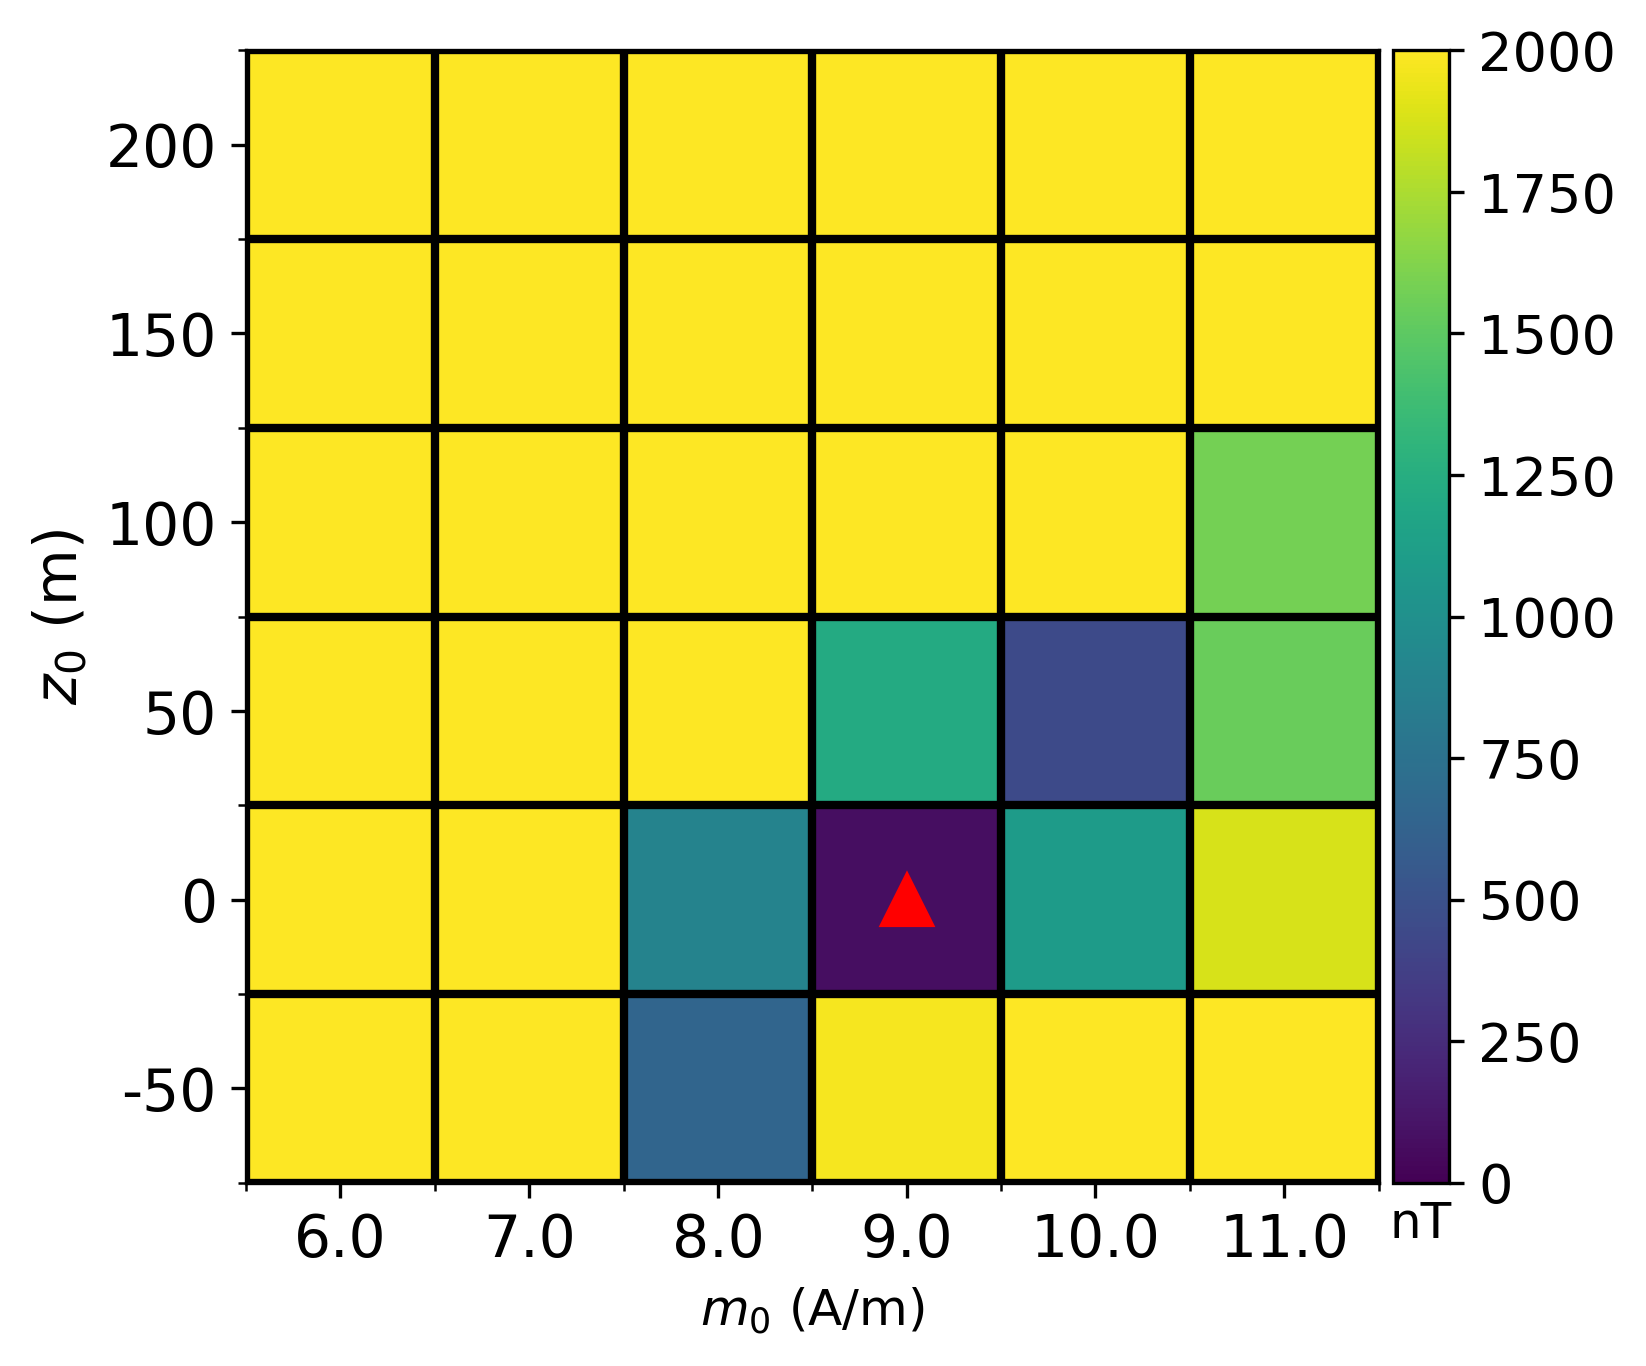
\includegraphics[scale=.75]{figures/simple_gamma.png}
%	\caption{Application to the simple model data. 
%	Discrete mapping of the goal function $\Gamma(\mathbf{p})$ (eq. \ref{eq:gamma}) on the plane $ m_0 \times z_0 $,  
%	produced by estimated models with different depths-to-the-top ($ z_0 $) and 
%	total-magnetization intensities ($ m_0 $). 
%	The red triangle represents the $m_0$ and $z_0$ of the true source.}
%	\label{fig:simple_map}
%\end{figure}

\begin{figure}
	\centering
	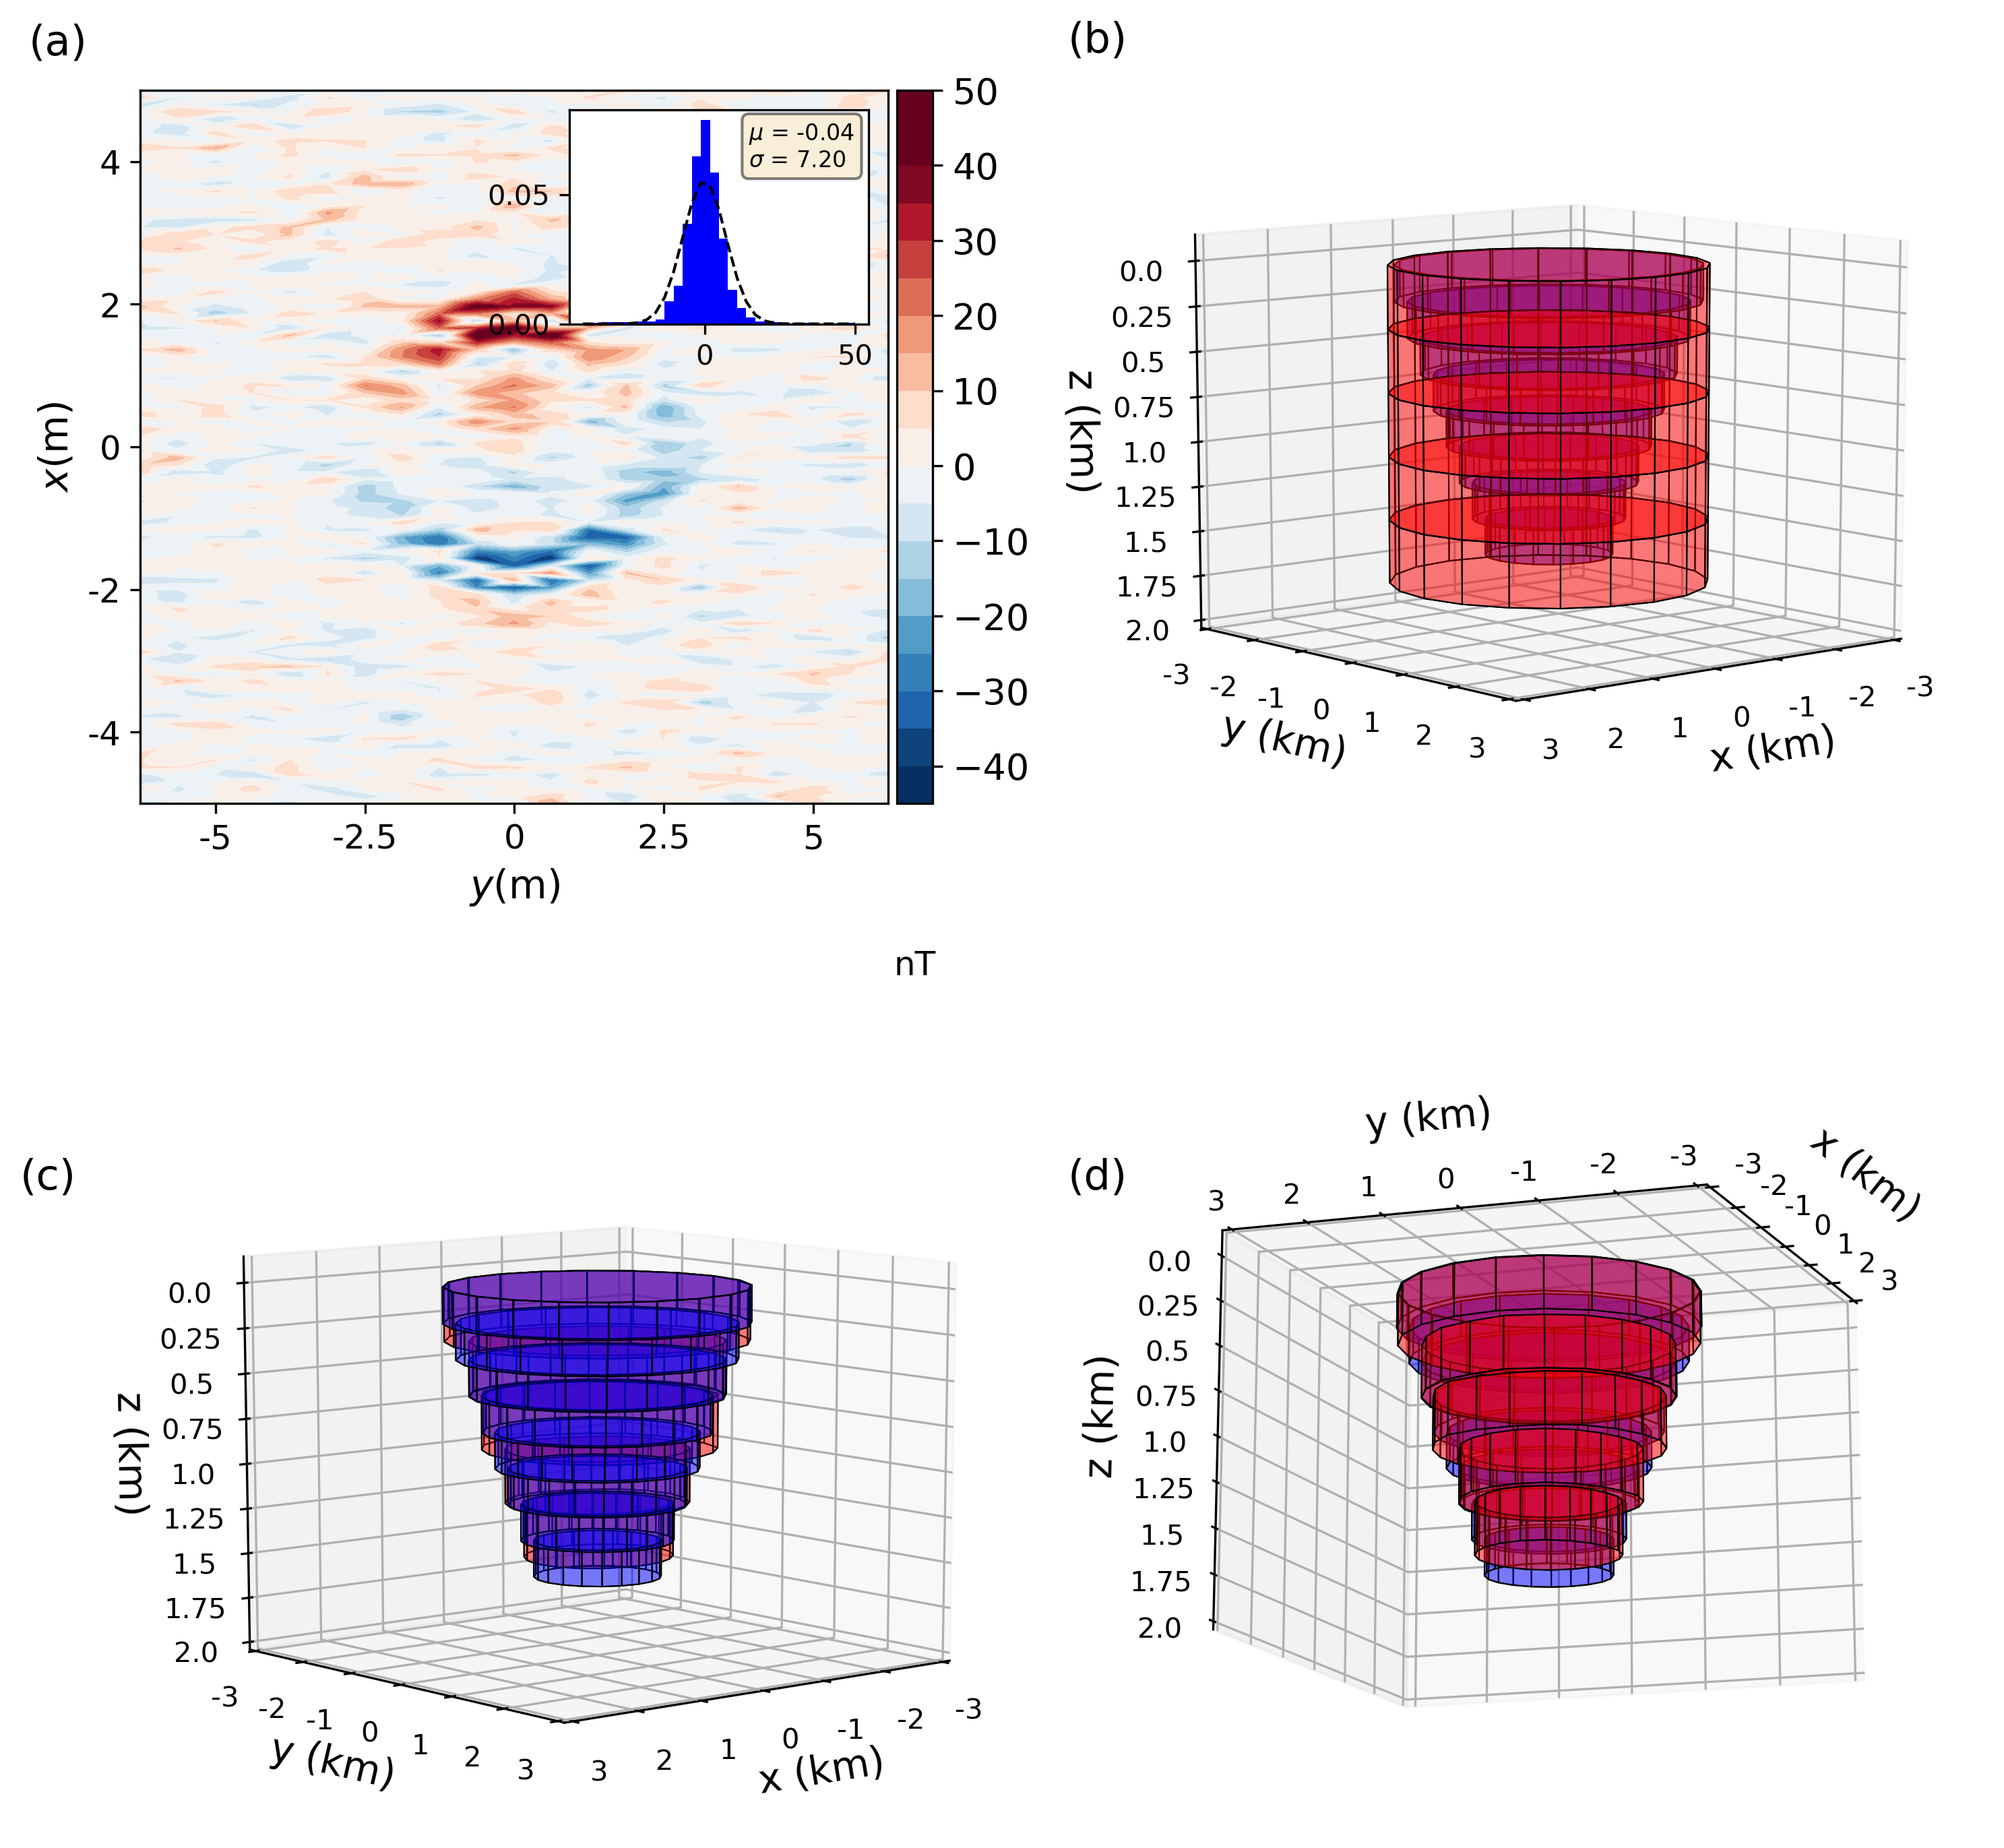
\includegraphics[width=\linewidth]{figures/simple_results.png}
	\caption{Application to the simple model data. (a) Residuals between the  noise-corrupted data (Fig. \ref{fig:simple_model}a) and the predicted data (not shown) produced by the estimated model (red prisms shown in the panels c and d). The inset in (a) shows the histogram of the residuals and the Gaussian curve (dashed line) has mean and standard deviation equal to $\mu = -0.04$ nT and $\sigma=7.21$ nT, respectively. (b) Perspective views of the initial approximation (red prisms) and the true model (blue prisms). (c) and (d) Comparison between the estimated source (red prisms) and the true model (blue prisms) in perspective views.}
	\label{fig:simple_results}
\end{figure}

% Application to synthetic data - complex model

\begin{figure}
    \centering
    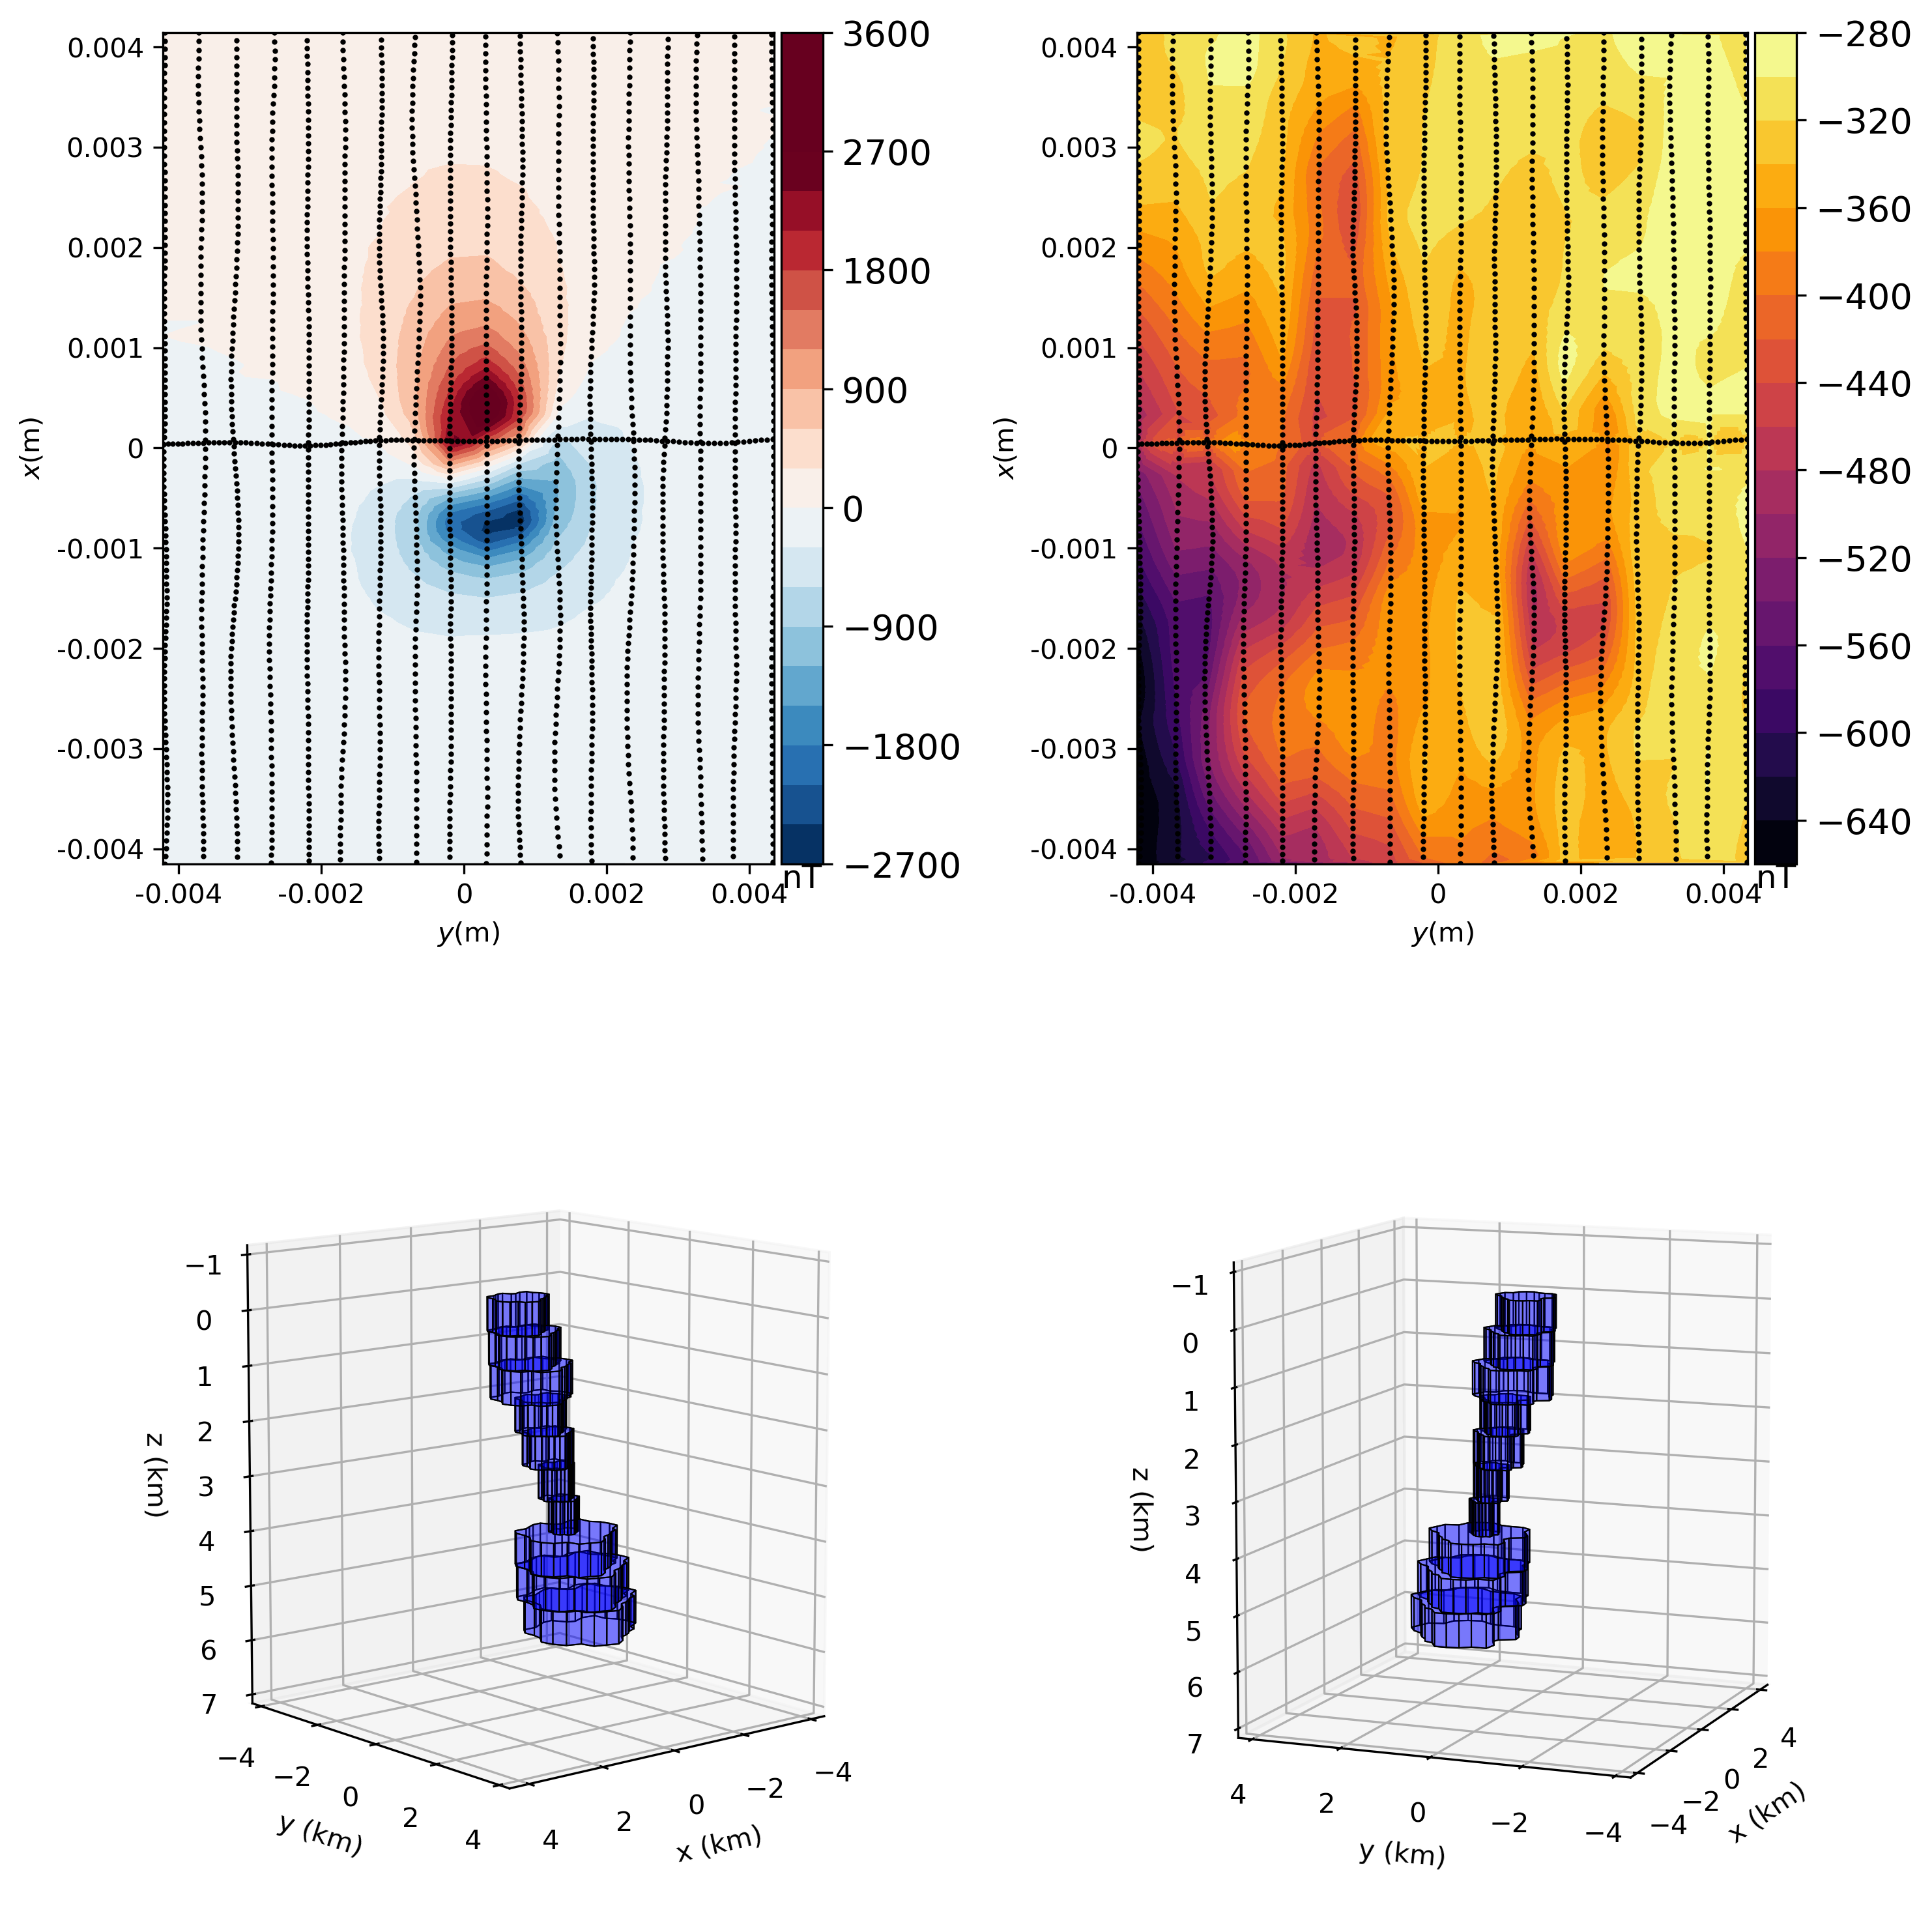
\includegraphics[width=\linewidth]{figures/complex_model_data.png}
    \caption{Complex model simulation. (a) Noise-corrupted total-field anomaly produced by the complex model (blue prisms shown in the panels c and d). The black dots represent the observation points. The connected red dots represent the horizontal projection 
   	of the initial approximation $\hat{\mathbf{p}}_{(0)}$ 
   	(red prisms in Fig. \ref{fig:complex_result}b). (b) Vertical coordinates of the observations simulating an airborne survey. (c) and (d) Perspective views of the complex model represented by the blue prisms.
}
    \label{fig:complex_model}
\end{figure}

%\begin{figure}
%	\centering
%	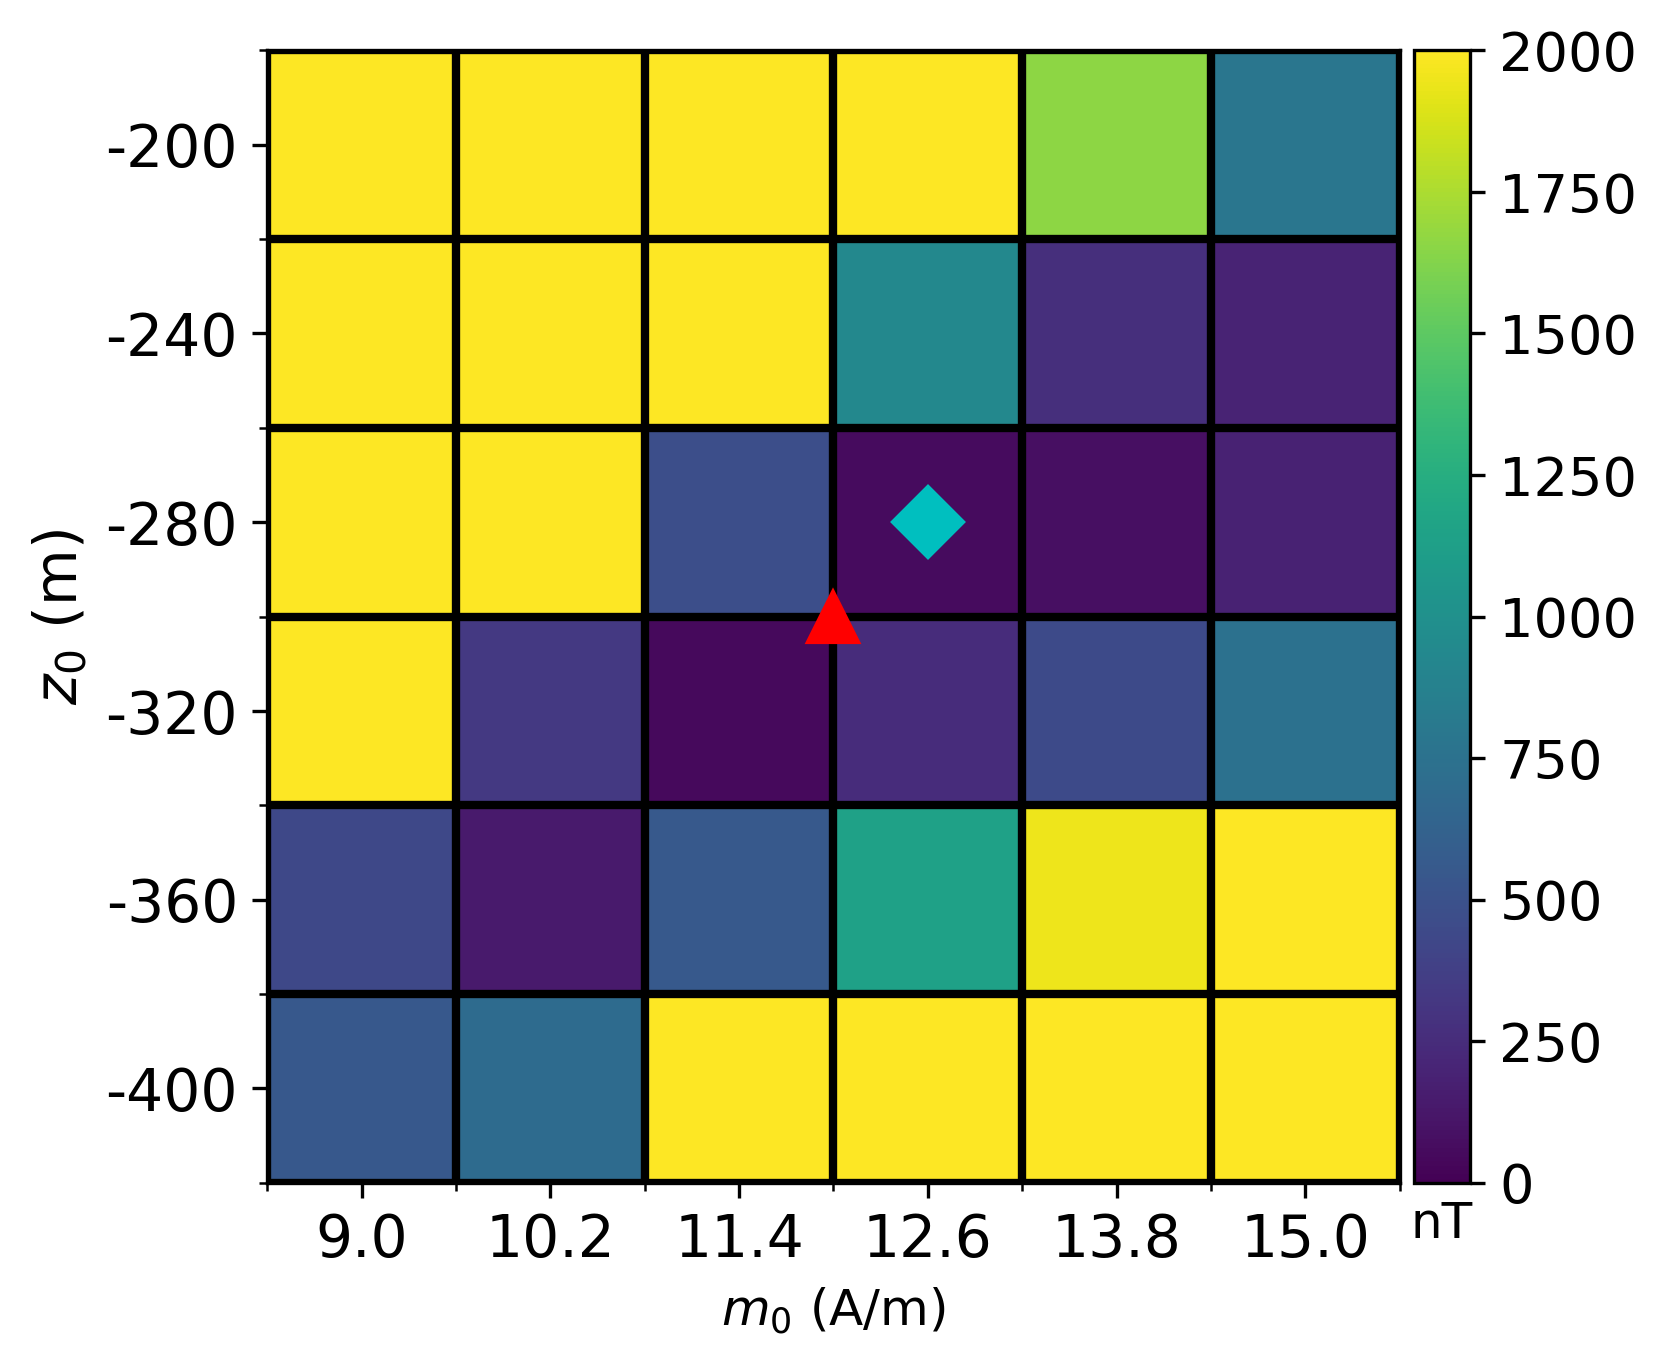
\includegraphics[scale=.75]{figures/complex_gamma.png}
%	\caption{Application to the complex model data. 
%	Discrete mapping of the goal function $\Gamma(\mathbf{p})$ (eq. \ref{eq:gamma}) on the plane $ m_0 \times z_0 $ produced by estimated models with different depths-to-the-top ($ z_0 $) and 
%	total-magnetization intensities ($ m_0 $). 
%	The red triangle represents the $m_0$ and $z_0$ of the true source. 
%	The white diamond indicates the pair ($ m_0, z_0 $) that produces the smallest 
%	value of $\Gamma (\mathbf{p})$.}
%	\label{fig:complex_map}
%\end{figure}

\begin{figure}
    \centering
    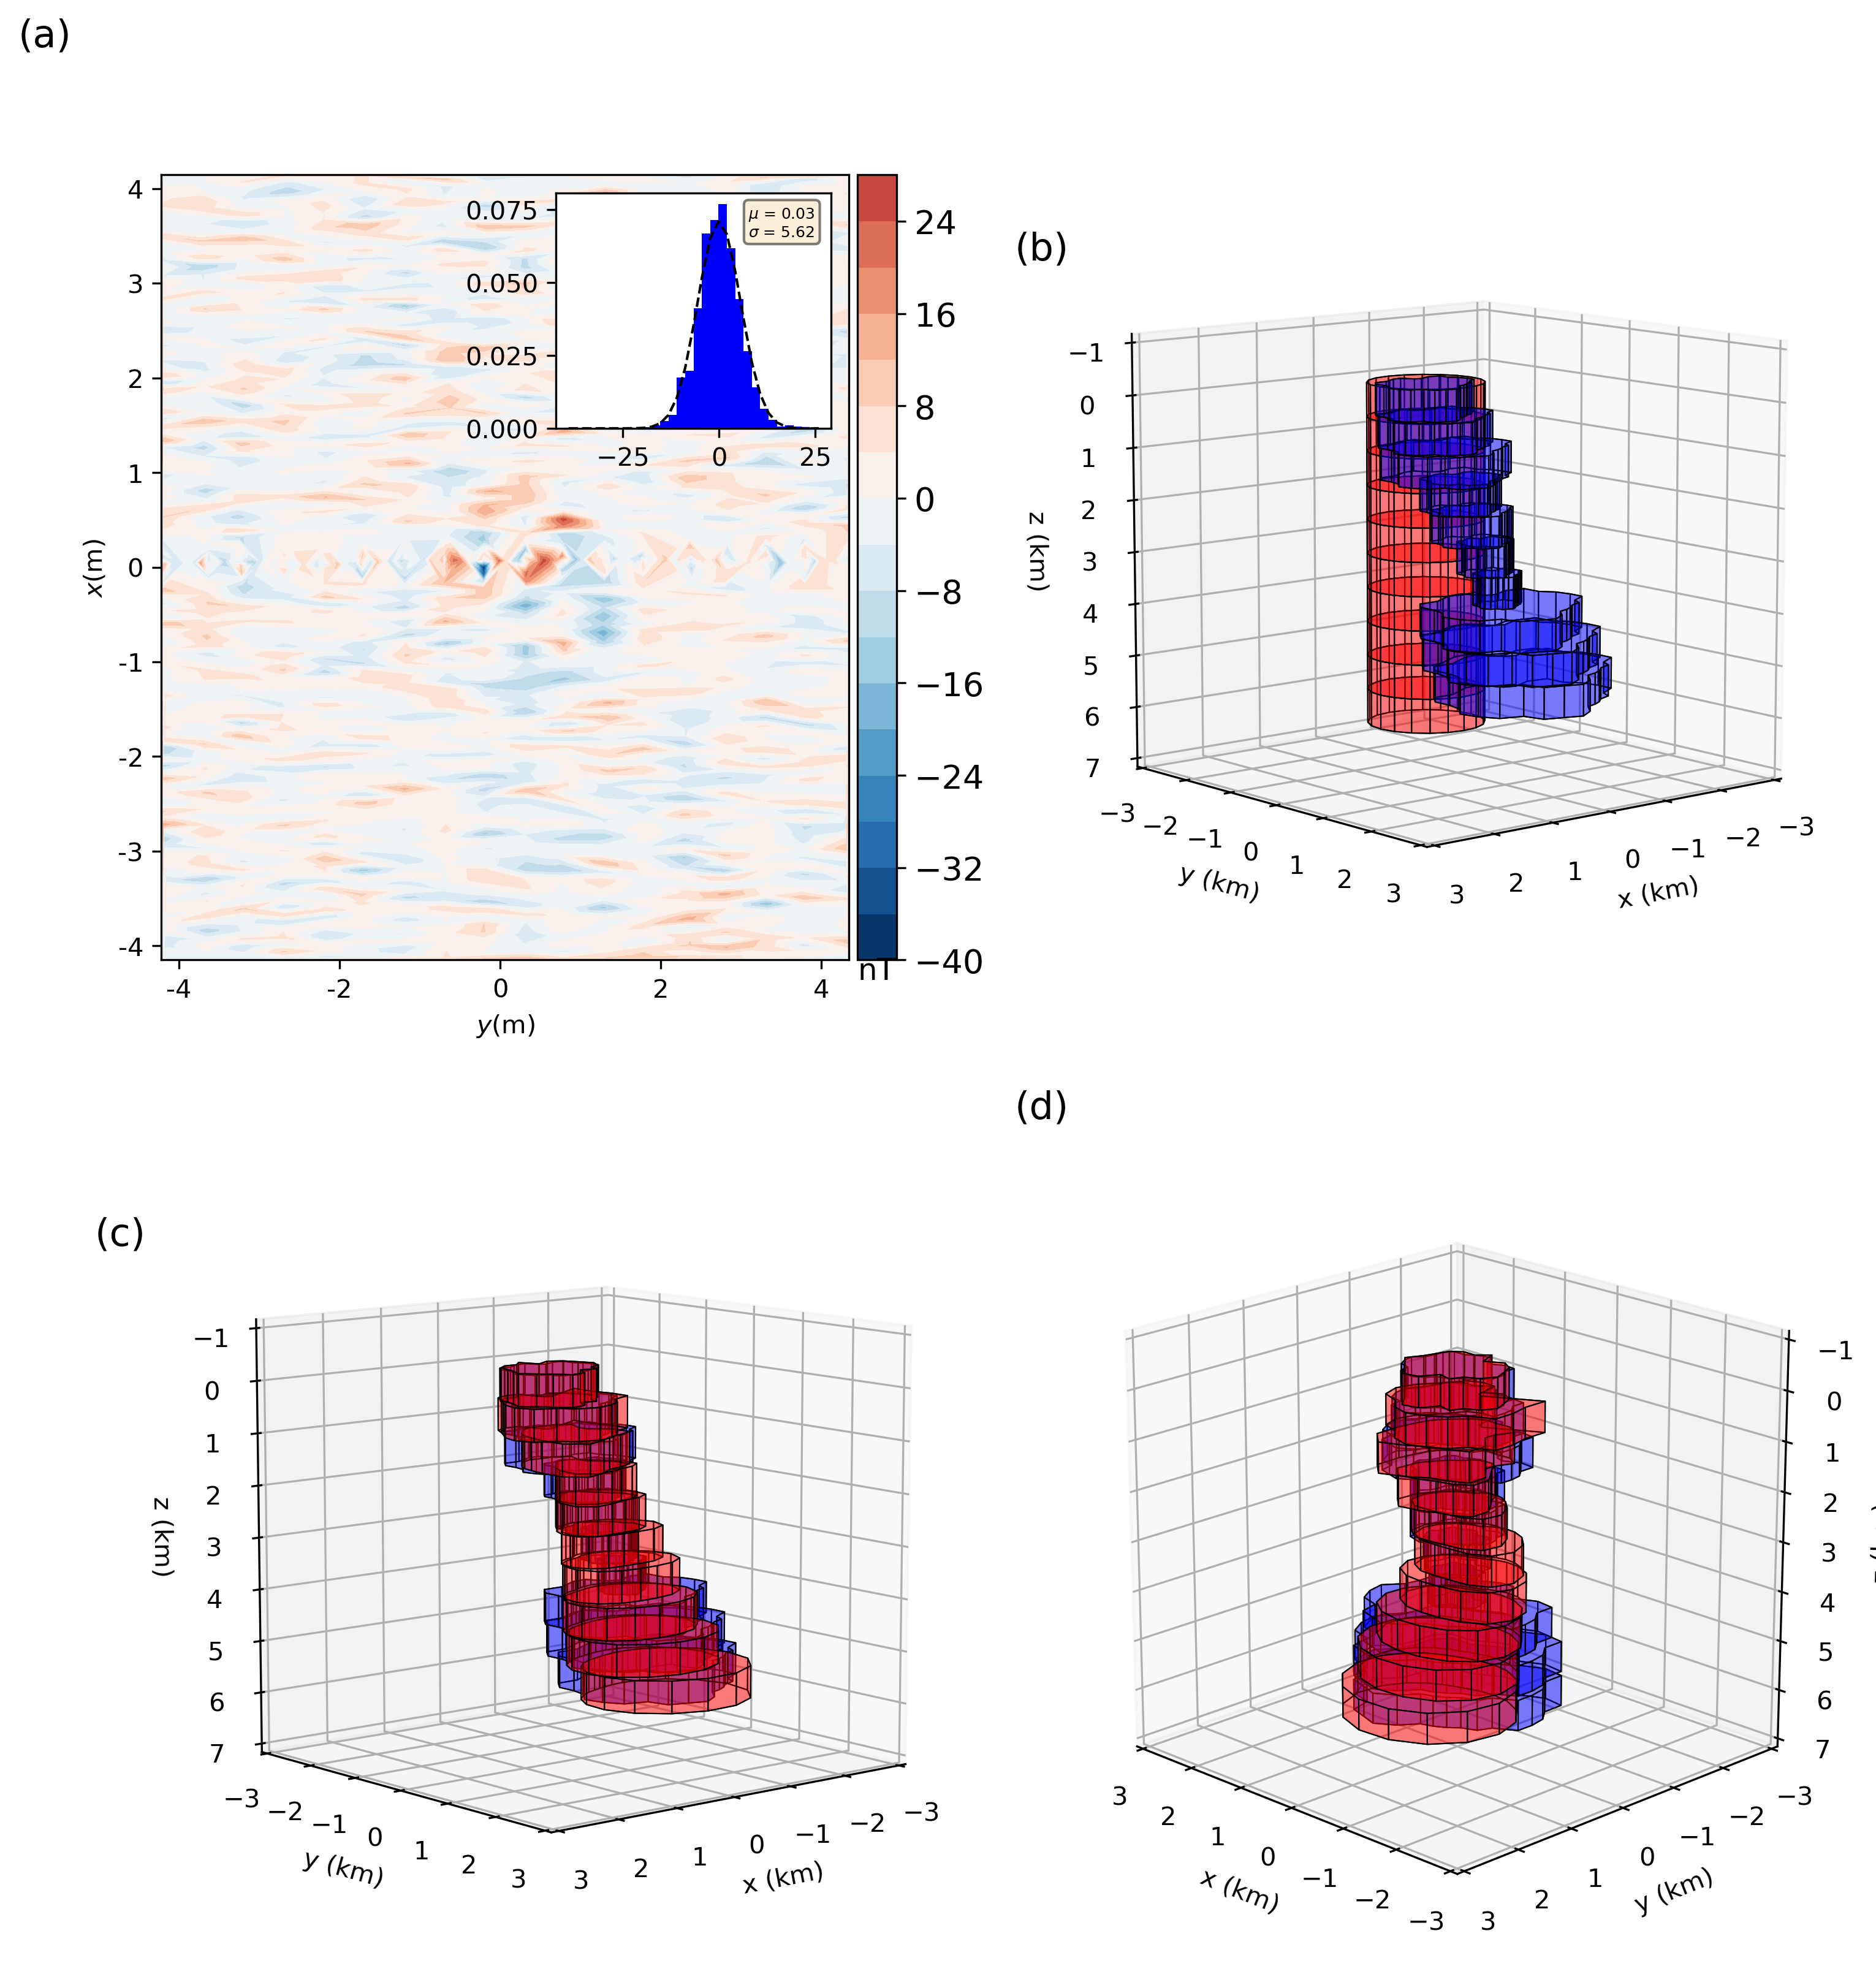
\includegraphics[width=\linewidth]{figures/complex_results.png}
    \caption{Application to complex model data. (a) Residuals between the noise-corrupted data (Fig. \ref{fig:complex_model}a) and the predicted data (not shown) produced by the estimated model (red prisms in the c and d panels). This model was obtained with 
    the values of $ m_0 $ and $ z_0 $ represented by the white diamond in Fig. \ref{fig:complex_map}. The inset in (a) shows the histogram of the residuals and the fitted Gaussian curve (dashed line) with mean and standard deviation equal to $\mu = 0.07$ nT and $\sigma=6.75$ nT, respectively. (b) Perspective view of the initial approximation (red prisms) and the true model (blue prisms). (c) and (d) Comparison between the estimated source (red prisms) and the true model (blue prisms) in perspective views. 
}
    \label{fig:complex_result}
\end{figure}

% Application to field data

\begin{figure}
    \centering
    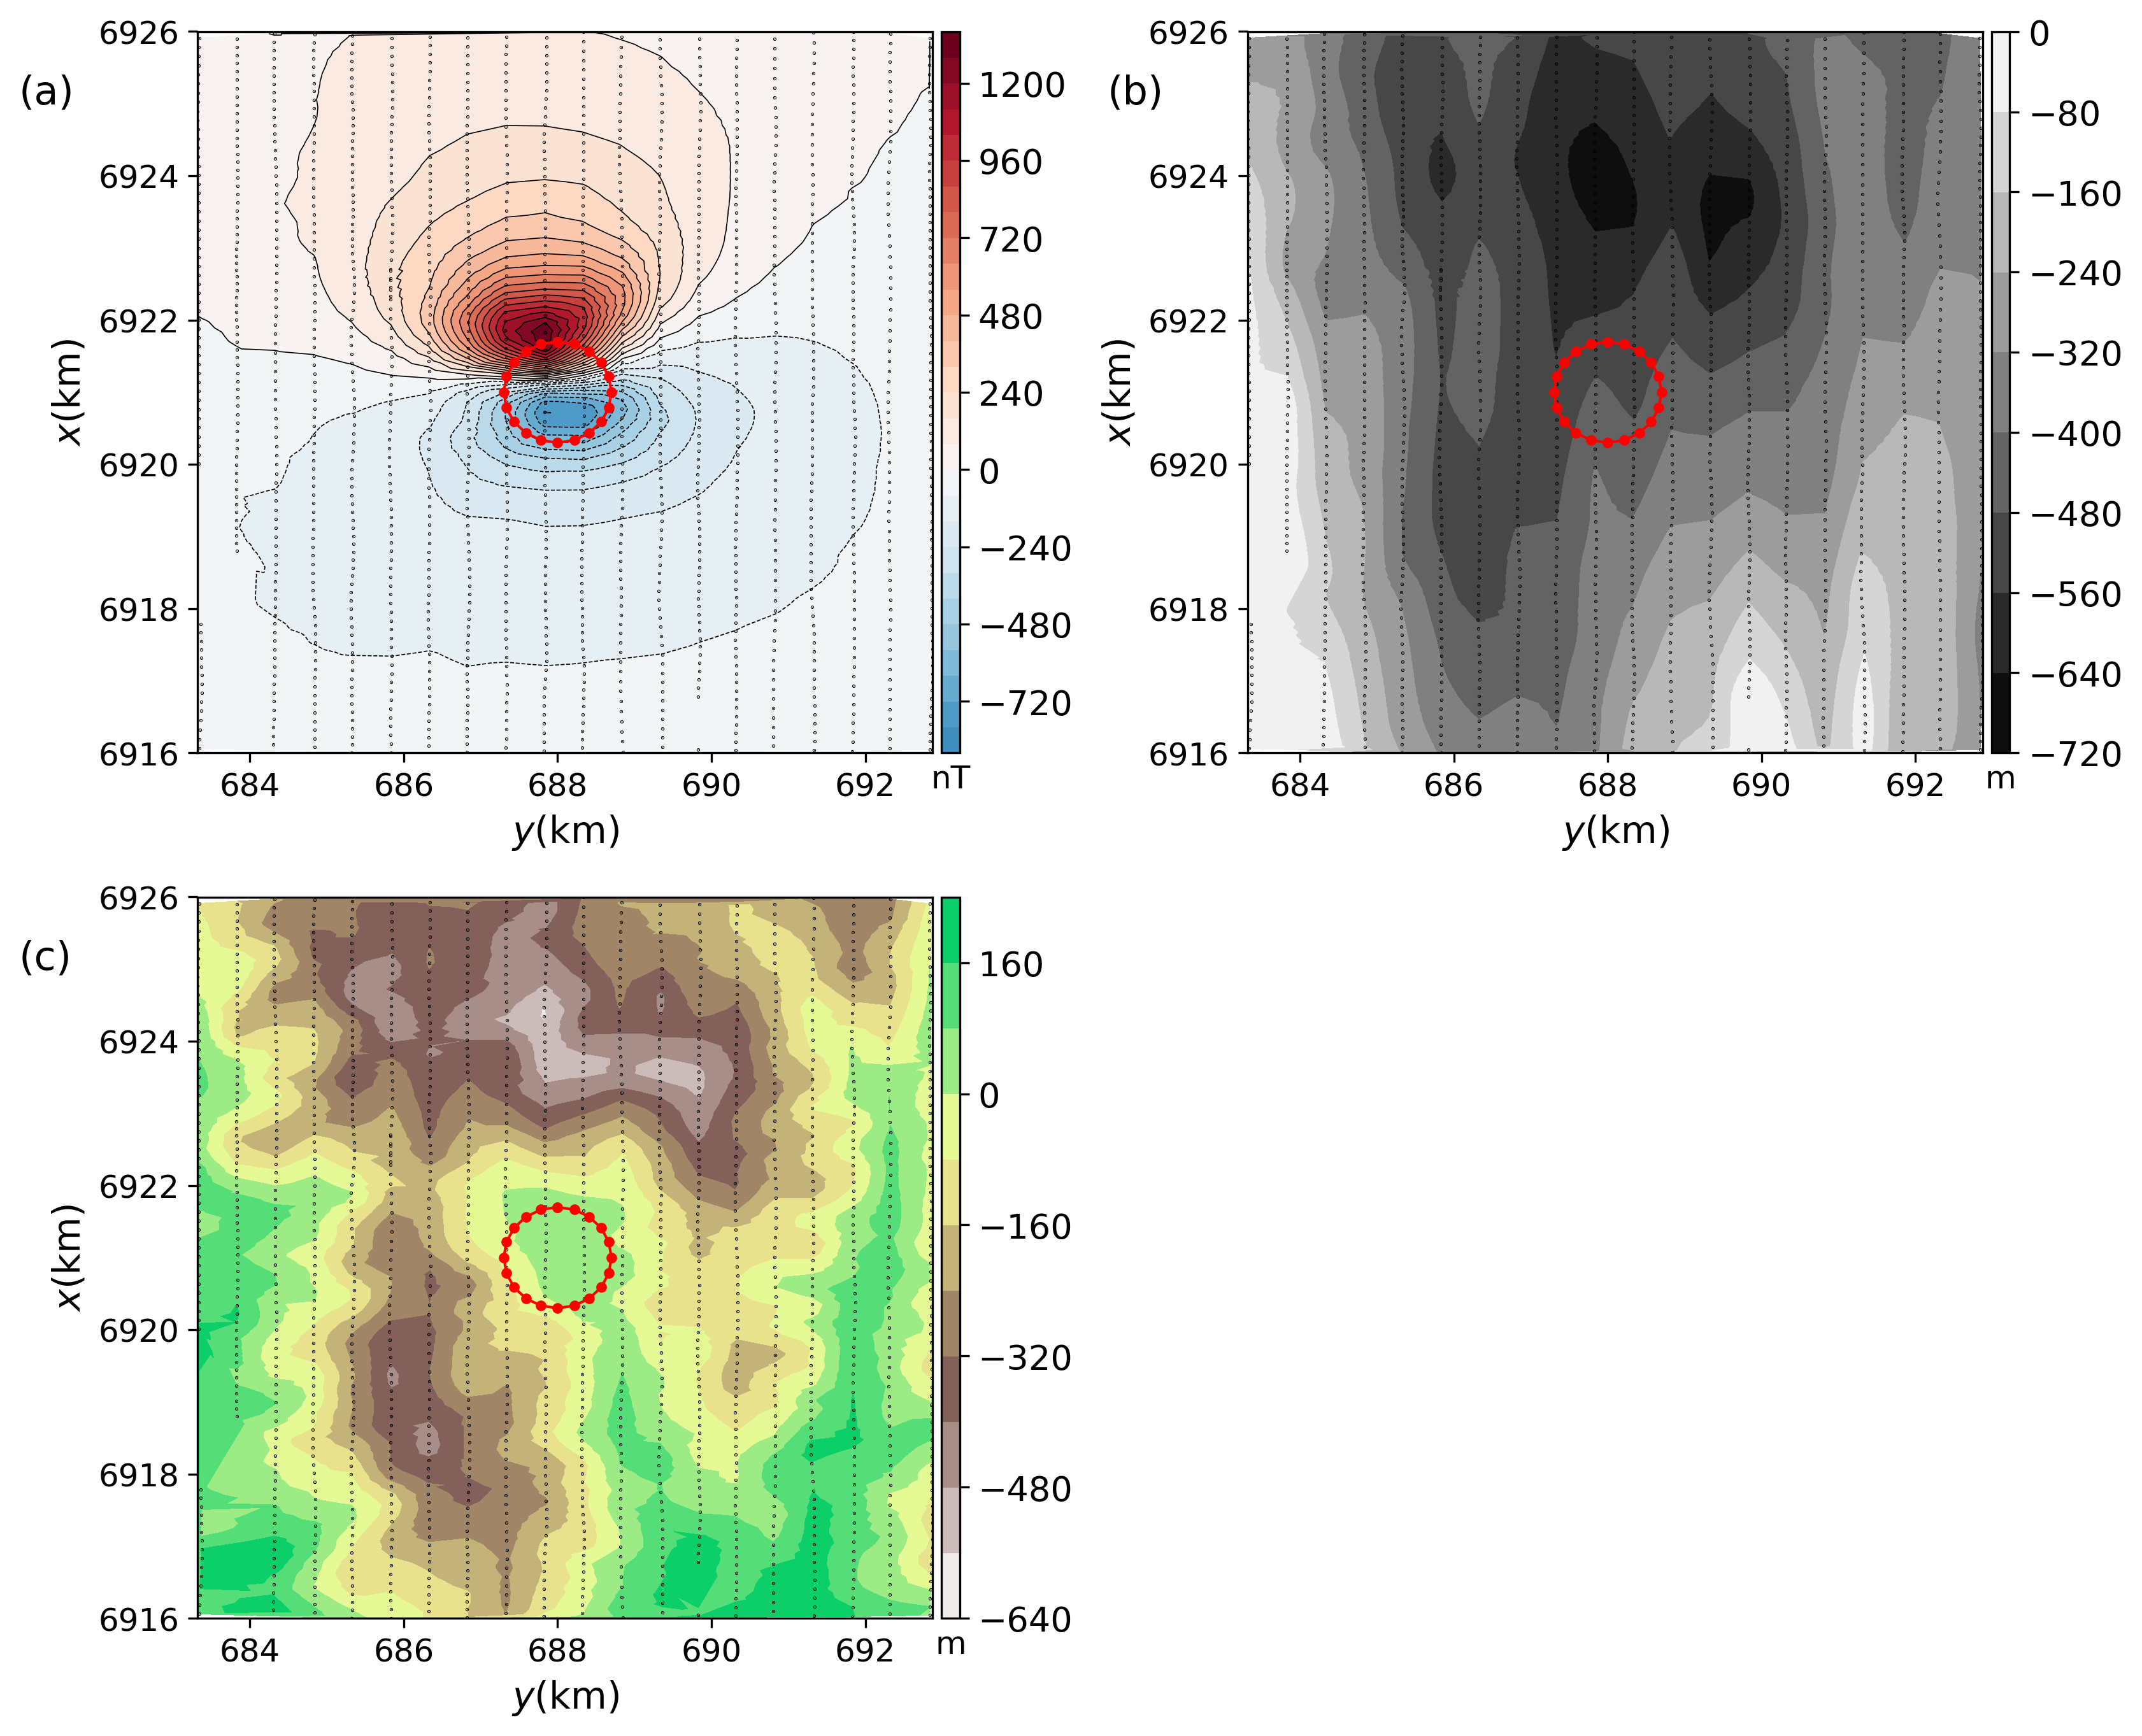
\includegraphics[width=\linewidth]{figures/field_data_alt_topo.png}
    \caption{(a) Residual total-field anomaly (in nT) over the  
    Anit{\'a}polis complex in southern Brazil. The horizontal UTM 
    coordinates are referred to the central meridian $ 51^\circ $ W. (b) Geometric 
    height of the observation points and (c) topography of the study area.
    Both of them are referred to the WGS84 ellipsoid. For convenience, we have 
    subtracted $ 800 $ m from their values. 
    The black dots represent the observation points. 
    The connected red dots represent the horizontal projection of the 
    initial approximation $\hat{\mathbf{p}}_{(0)}$ 
    (red prisms in Figs \ref{fig:real_result2}b and \ref{fig:real_result}b).}
    \label{fig:real_data}
\end{figure}

%\begin{figure}
%	\centering
%	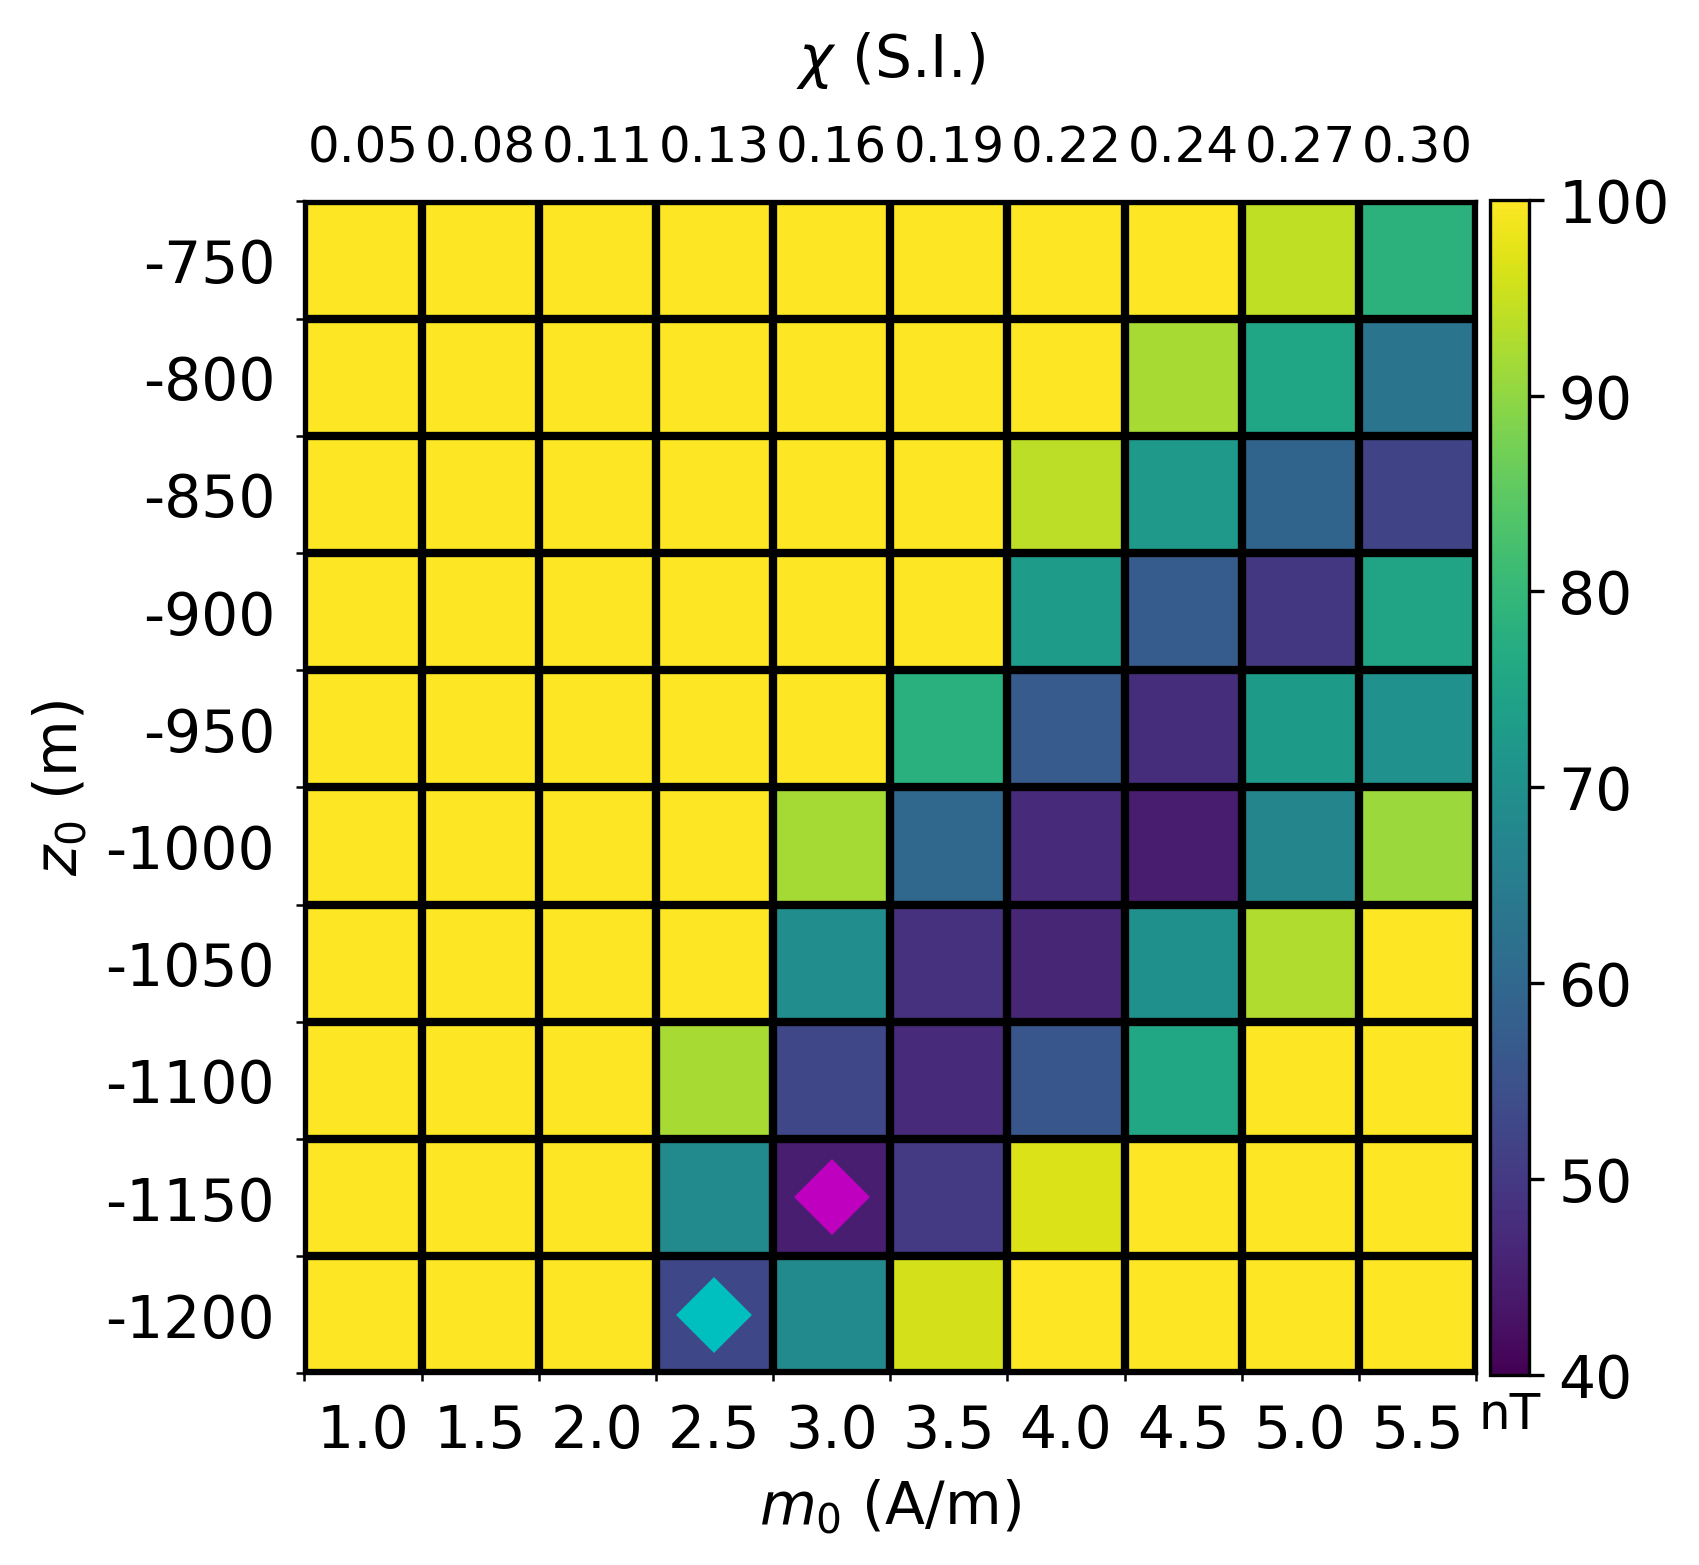
\includegraphics[scale=.75]{figures/real_gamma.png}
%	\caption{Application to the field data over the Anit{\'a}polis complex in southern Brazil. 
%	Discrete mapping of the goal function $\Gamma(\mathbf{p})$ (eq. \ref{eq:gamma})  
%	produced by estimated models with different depths-to-the-top ($ z_0 $) and 
%	total-magnetization intensities ($ m_0 $).
%	The pink diamond represents the estimated model that produces the smallest value of $ \Gamma(\mathbf{p})$.
%	The white diamond represents an alternative model whose depth to the top is $z_0=0$ indicating a possible outcropping not corroborated by the literature.}
%	\label{fig:real_map}
%\end{figure}

\begin{figure}
	\centering
	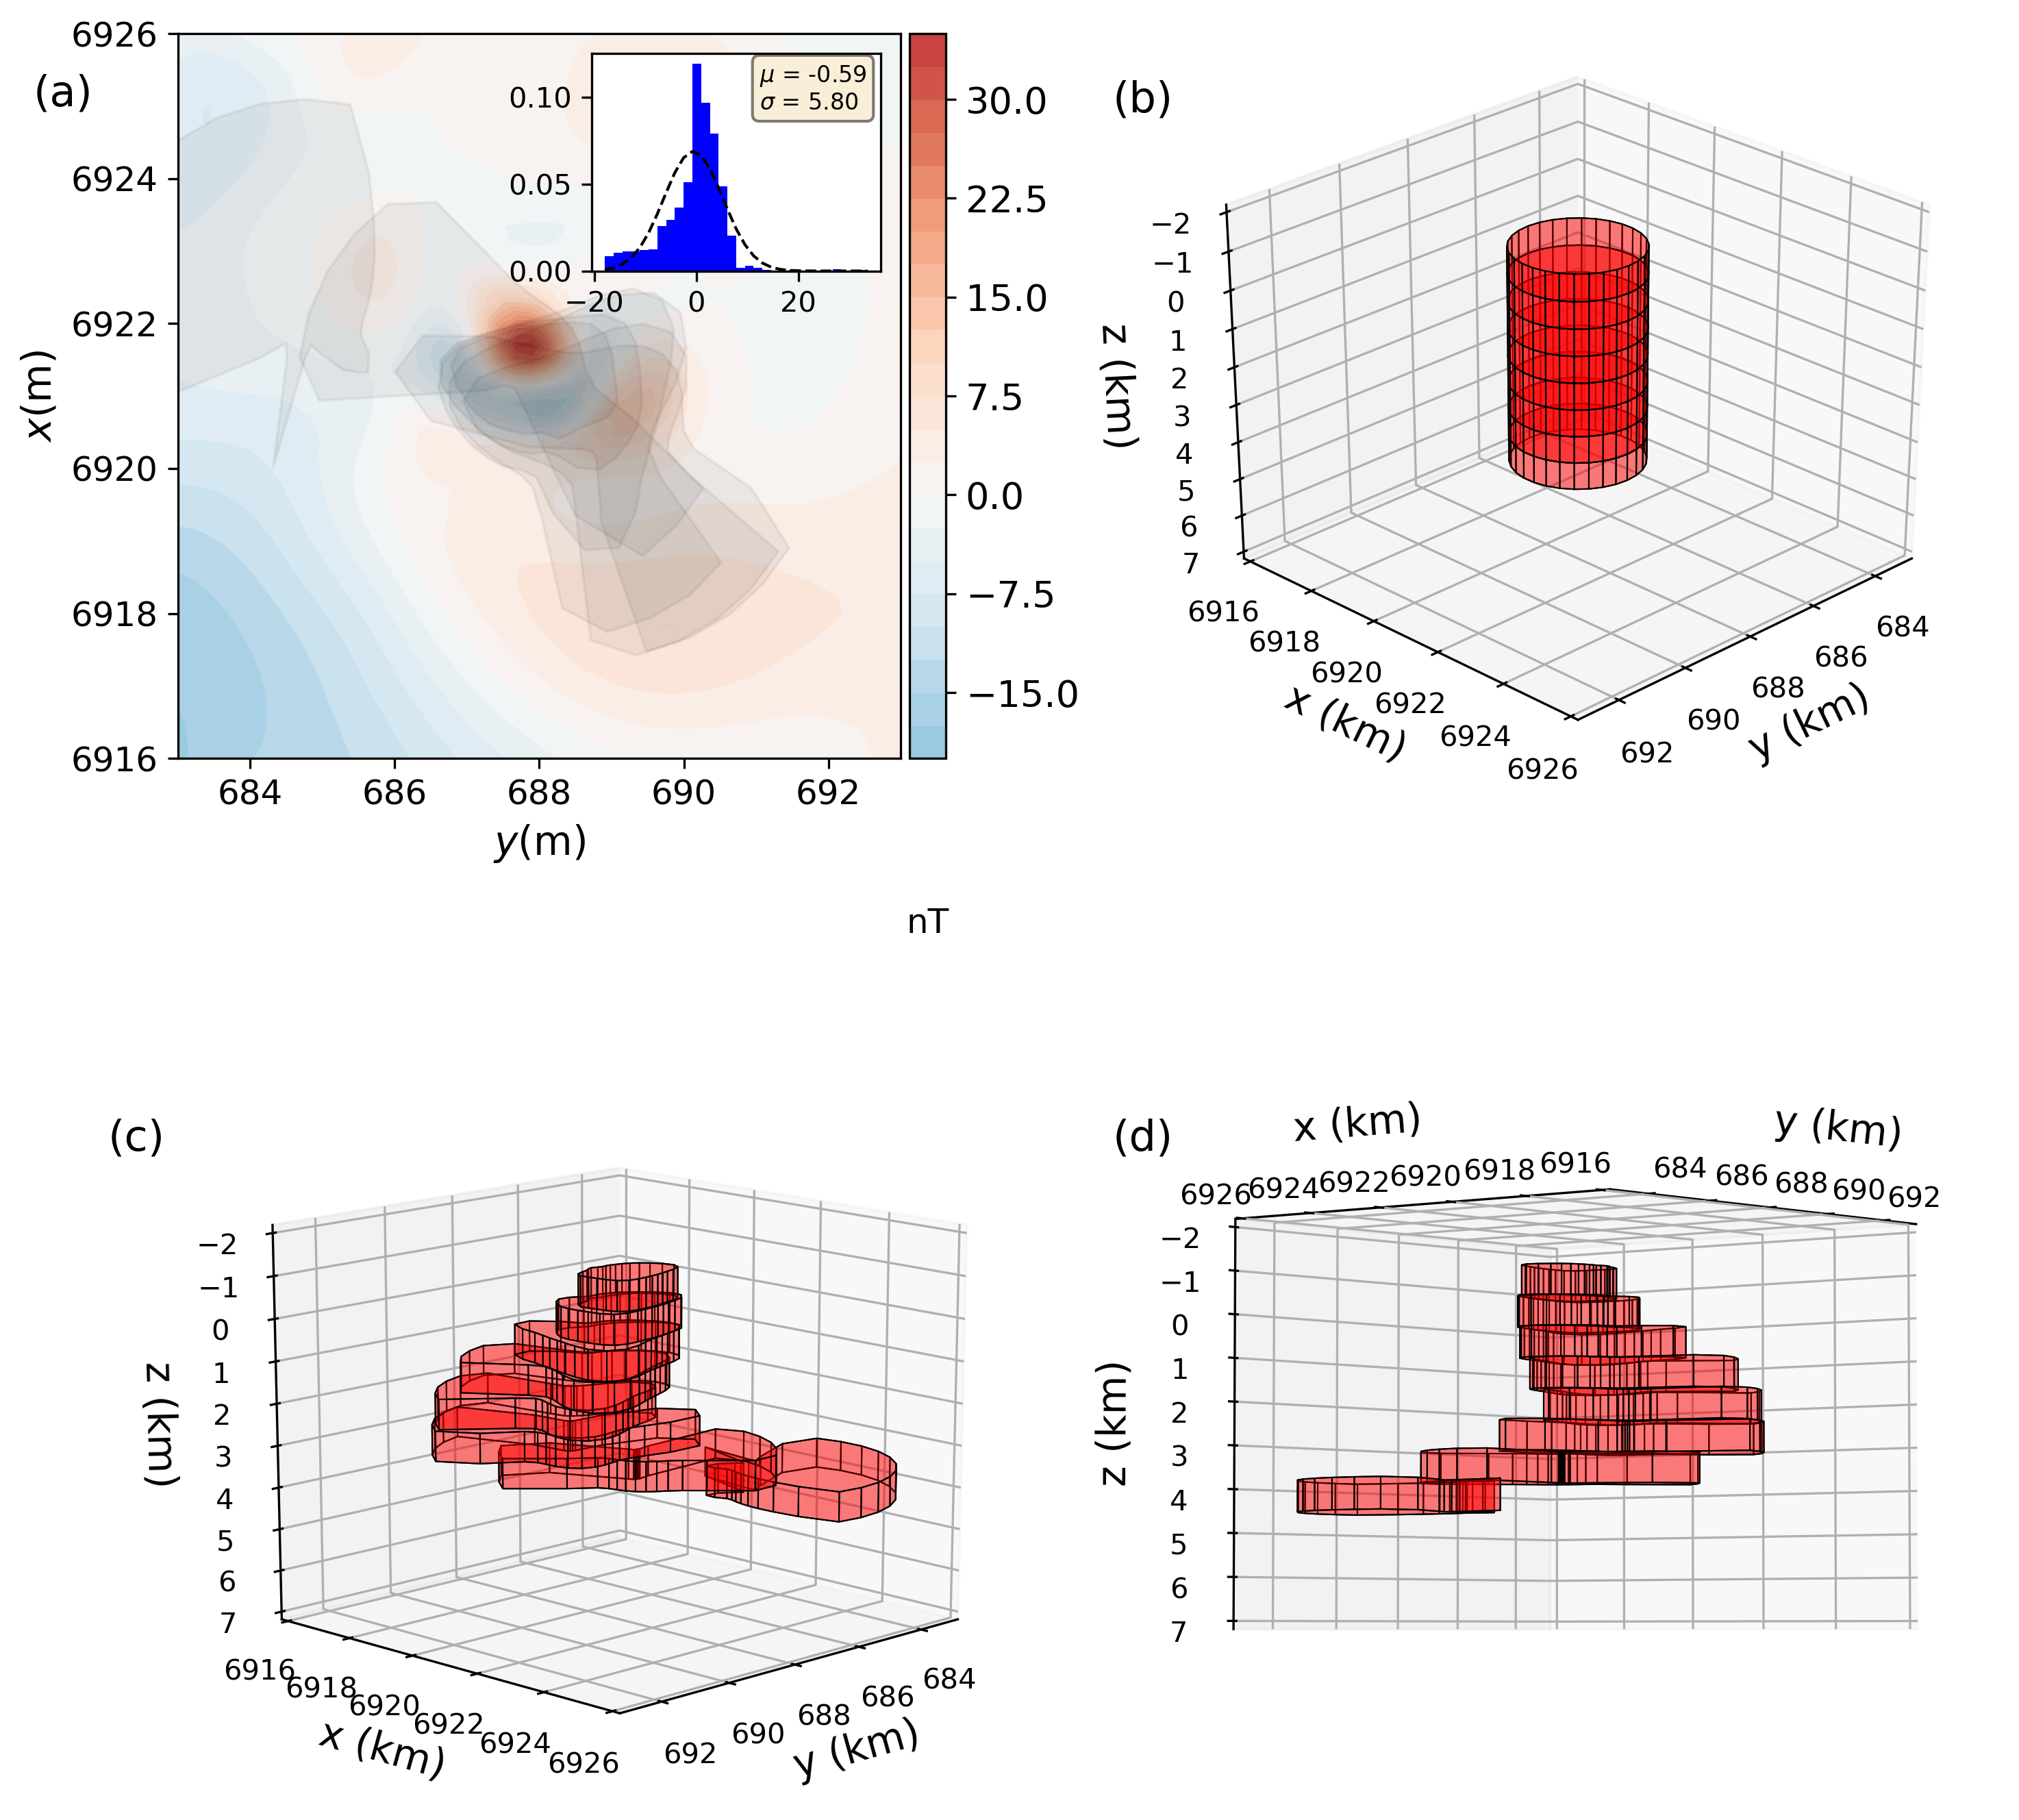
\includegraphics[width=\linewidth]{figures/real_results_magenta_diamond.png}
	\caption{Application to the field data over the Anit{\'a}polis complex, Brazil.
	The non-outcropping estimated model producing the smallest goal function value, 
	represented by the pink diamond in Fig. \ref{fig:real_map}.
	(a) Residuals between the observed data (Fig. \ref{fig:real_data}a) and the 
	predicted data (not shown) produced by the estimated model. 
	The inset shows the histogram of the residuals and the fitted normal 
	Gaussian curve (dashed line) with mean $\mu = -2.53$ nT and standard deviation $\sigma = 22.70$ nT.
	The light-gray polygons represent the horizontal projection of the estimated 
	model onto the residual map. 
	(b) Perspective view of the initial approximation (red prisms). 
	(c) and (d) Perspective views of the estimated model (red prisms).}
	\label{fig:real_result2}
\end{figure}

\begin{figure}
    \centering
    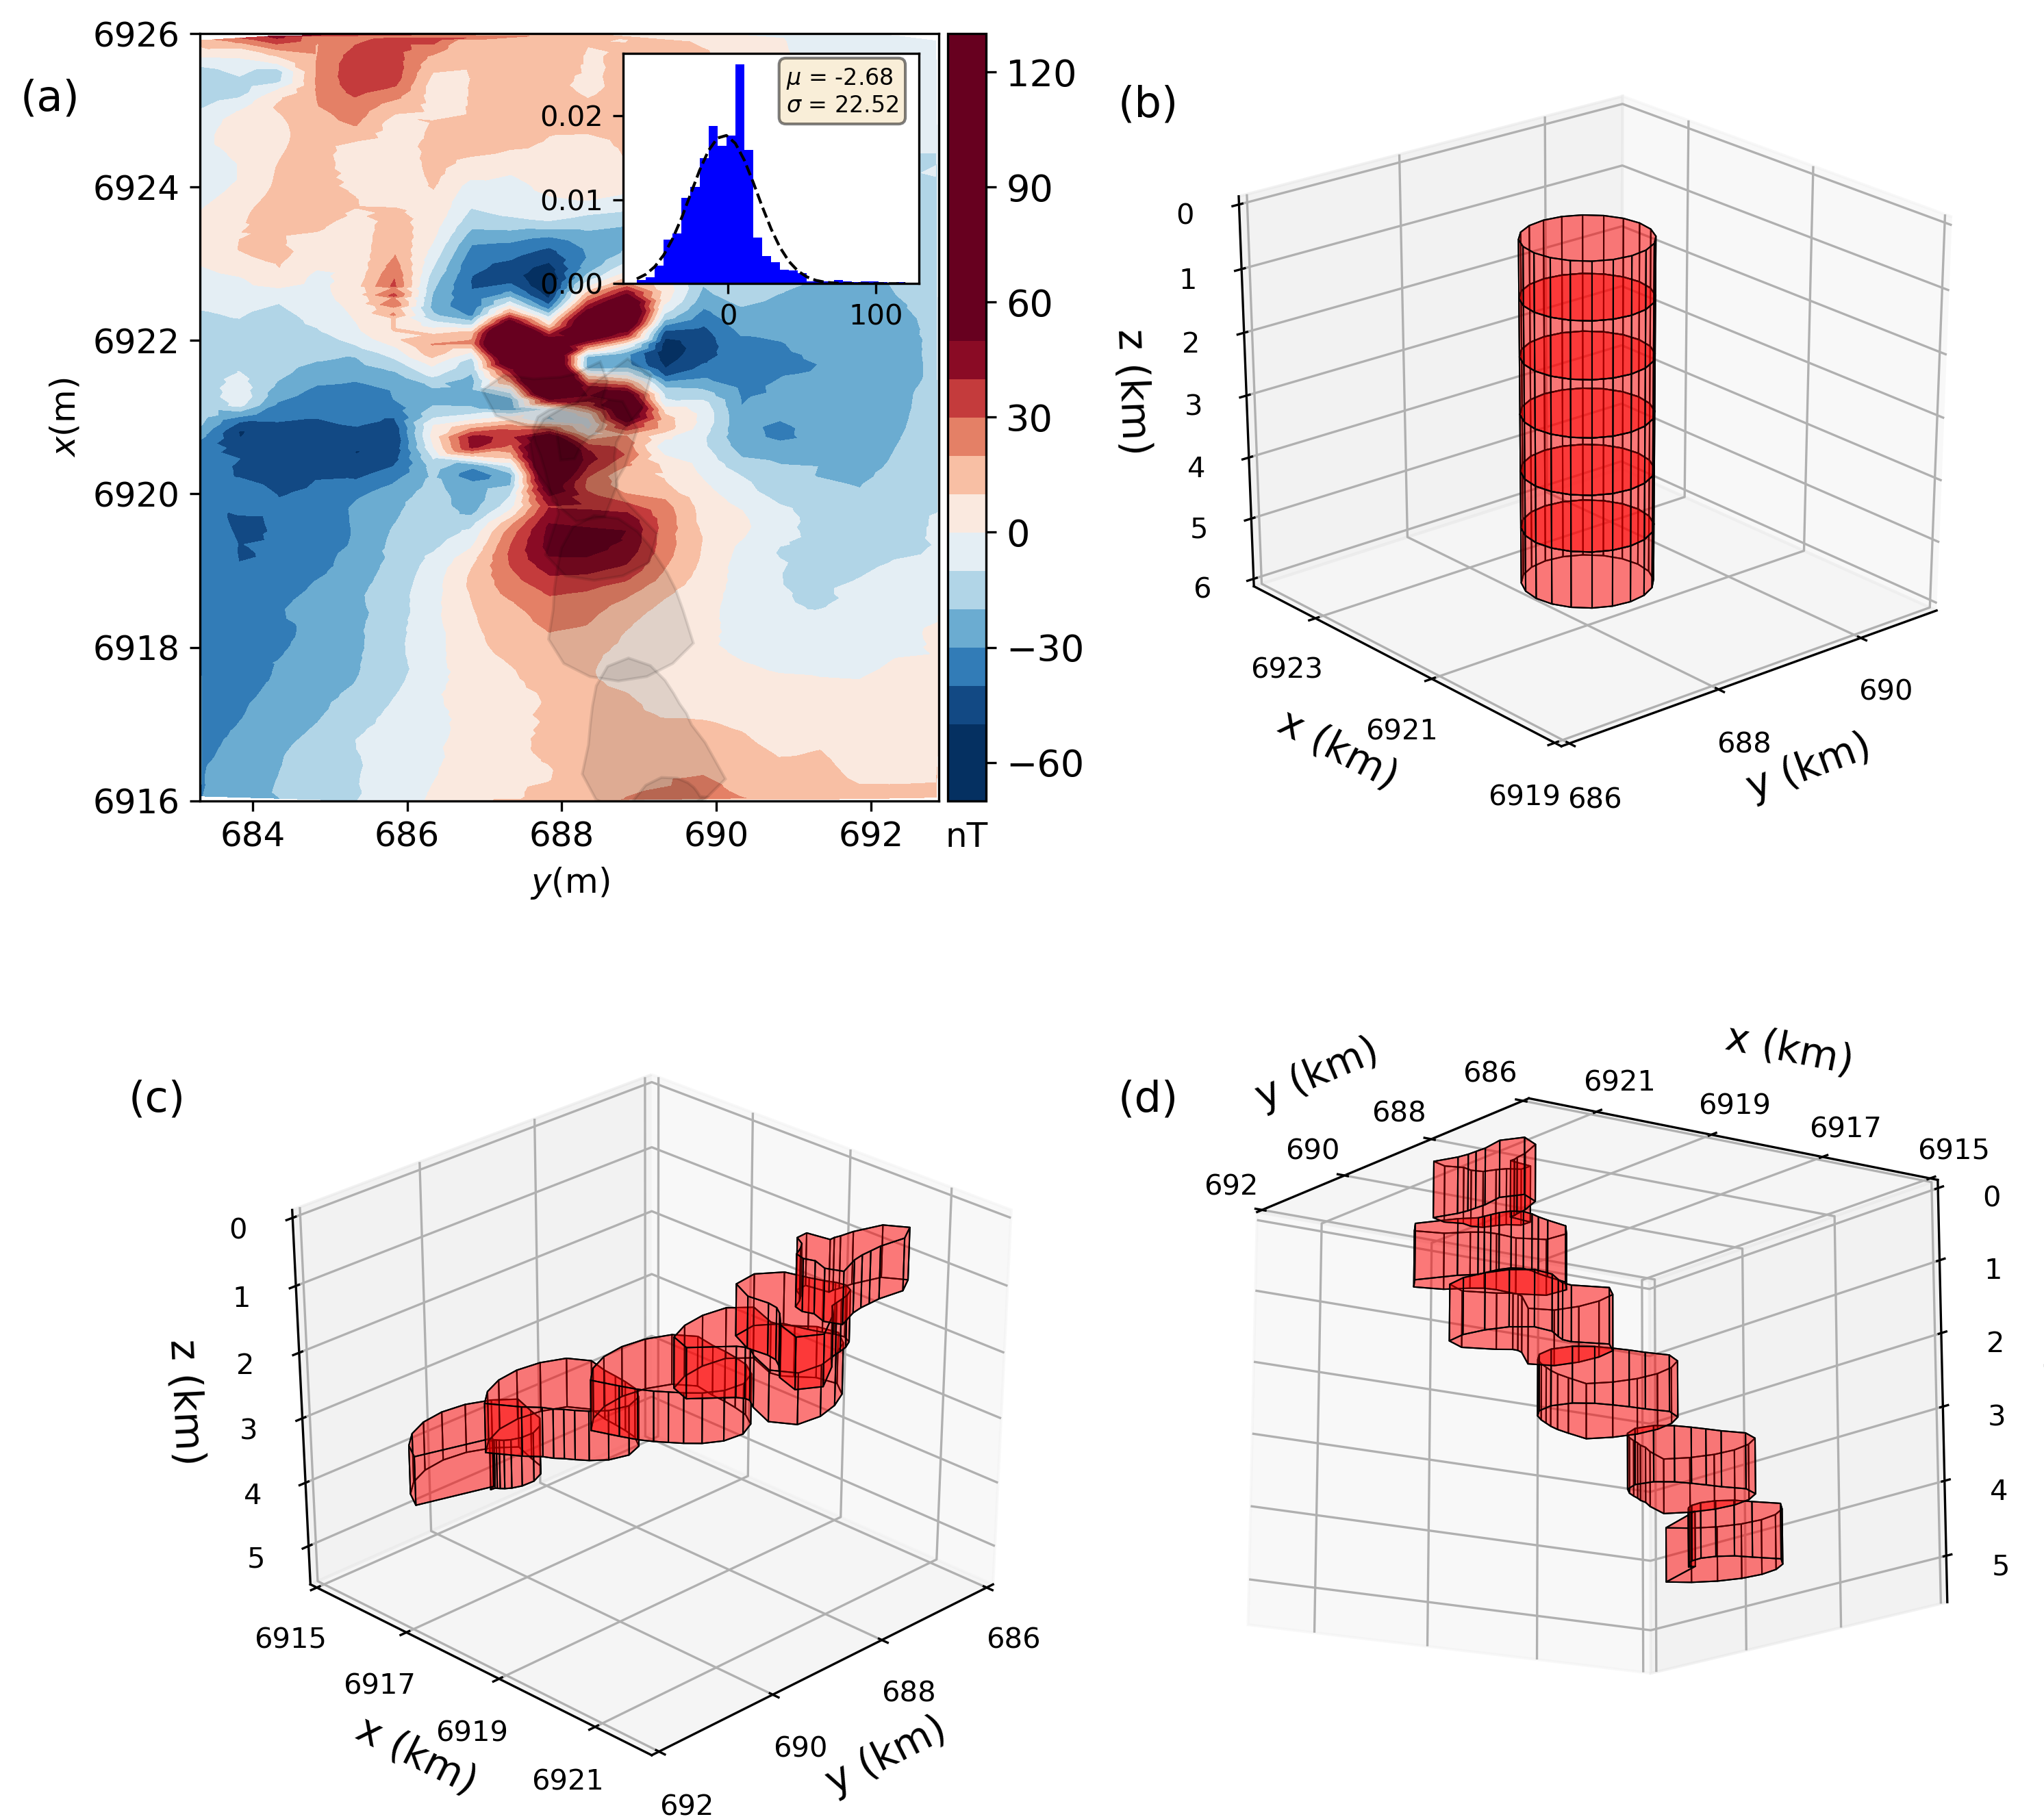
\includegraphics[width=\linewidth]{figures/real_results_white_diamond.png}
    \caption{Application to the field data over the Anit{\'a}polis complex, Brazil.
    Outcropping estimated model 
    represented by the white diamond in Fig. \ref{fig:real_map}. 
    (a) Residuals between the observed data (Fig. \ref{fig:real_data}a) and the 
    predicted data (not shown) produced by the estimated model. 
    The inset shows the histogram of the residuals and the fitted normal 
    Gaussian curve (dashed line) with mean $\mu = -2.68$ and standard deviation  $\sigma = 22.52$.
    The light-gray polygons represent the horizontal projection of the estimated 
    model onto the residual map. 
    (b) Perspective view of the initial approximation (red prisms). 
    (c) and (d) Perspective views of the estimated model (red prisms).}
    \label{fig:real_result}
\end{figure}